\chapter{A complete pipeline for user adaptation}
\label{chapter:sigdial}

\section{Motivation}

In this chapter, we tackle the problem  of fast optimisation of \idx{user}-adapted \idx{dialogue} strategies by means of \acrfull{RL} as stated in \Cref{chapter:dm-tl} . The main goal is to improve \idx{jumpstart} learning of \gls{RL}-based \idx{dialogue} management strategies when facing new users\index{user}, by transfering\index{transfer} data collected from similar \idx{user}s~\parencite{Lazaric2008}\index{user}. To do so, we consider the setting in which a large amount of \idx{dialogue}s have been collected from several users\index{user}, and a new user\index{user} connects to the service~\parencite{Genevay2016}. This solution combines techniques from the literature on \gls{MAB}~\parencite{auer2002}, \idx{batch} \gls{RL}~\parencite{Ernst05,Lihong09,Chandramohan2010,pietquin2011sample} and \idx{policy}/\gls{MDP} \idx{clustering}~\parencite{Chandramohan2012,mahmud2013}.

Instead of \idx{clustering} \idx{user} behaviours as in \textcite{Chandramohan2012}, we propose to cluster the policies that are trained on the \idx{user} \idx{dialogue} datasets. To do so, we define a novel \idx{policy}-based distance, called \textsc{PD-Distance}. Then, we investigate several \idx{clustering} methods: $k$-medoids~\parencite{kmedois} and $k$-means~\parencite{kmeans,macqueen1967some}, which enable the identification of \textit{source representatives} for the \acrfull{TL}. Once clusters representatives have been selected, they are plugged into a multi-armed bandit algorithm, as proposed in \textcite{Genevay2016}.

Following previous work where \idx{user adaptation} ~\parencite{janarthanam2010-tl-dialogue,Ultes2015} was used to address negotiation tasks~\parencite{Sadri2001,Georgila2011,Barlier2015,Genevay2016}, we test our methods on different types of \idx{user}s involved in a negotiation game~\parencite{Laroche2016}. Methods are compared with two baselines: learning without \idx{transfer} and \idx{transfer} from a generic \idx{policy} learnt from all the sources. These methods are tested by interacting with \idx{handcrafted user}s and \idx{human-model user}s learnt from actual human interactions (unlike ~\textcite{Genevay2016}). These experiments show that our \idx{clustering} methods provide a better \idx{dialogue} experience than the generic methods in both setups.

We present the full \idx{user adaptation} process in ~\Cref{sec:adapatationframework}. The \idx{clustering} methods are described in \Cref{sec:systemsrepresentatives}. \Cref{section:experiments-sigdial} describes the negotiation game and the experiments.


\section{Adaptation process}
\label{sec:adapatationframework}

\begin{figure}[b!]
    \bigcentering
    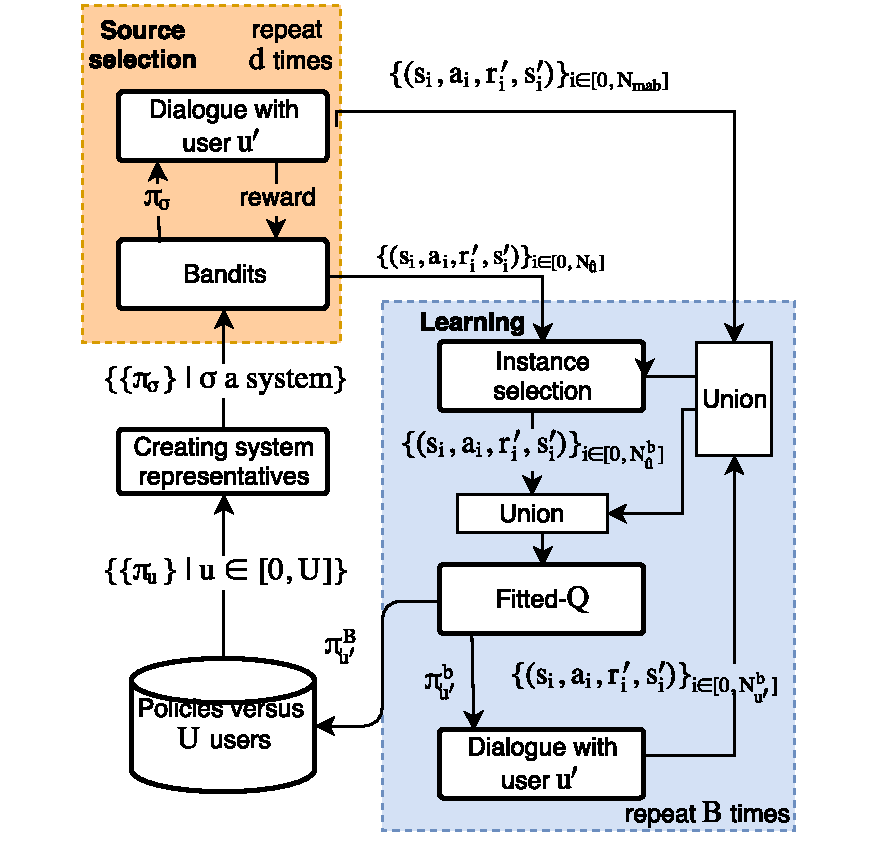
\includegraphics[width=0.9\columnwidth]{sources/contribution/sigdial/dataflow.pdf}
    \caption{Adaptation process}
    \label{fig:adaptationframework}
\end{figure}


\Cref{fig:adaptationframework} shows the full process of \idx{user adaptation}. As an input, we assume the existence of a database of \idx{dialogue}s with different source \idx{user}s, which allows the training of \idx{user} specialised policies. At first, the process consists in searching or constructing \idx{policy} representatives for this database so as to reduce the number of possible \idx{transfer} sources. This is where the contribution of this chapter mainly stands, the rest being mostly inherited from \textcite{Genevay2016}.

\subsection{The \textit{knowledge-transfer} phase}

The \textit{knowledge-transfer} phase is operated on two levels: the selection of a source policy (system) and the selection of the relevant transitions used to learn this source policy.

\paragraph{Source selection} The source selection problem is cast into a \gls{MAB} algorithm, implemented here as \gls{UCB}1~\parencite{auer2002}, each arm standing for a representative. When the \gls{MAB} selects an arm, its corresponding \idx{policy} $\policy$ interacts with the \idx{user} for one full \idx{dialogue}. The \gls{MAB} performs $n_{mab}$ \idx{policy} selections. $\T_{mab}$ \idx{transition}s from \idx{dialogue}s, with target \idx{user} $u'$, are collected during this procedure. In the end of this initial \gls{MAB} step, the representative \idx{policy} that yielded the highest empirical reward designates the source from which to \idx{transfer}. The algorithm \idx{transfer}s $\T_{\hat{u}}$ \idx{transition}s from its source $\hat{u}$ \idx{dialogue}s, to construct a \idx{batch} of dialogues\index{dialogue}. \idx{Transition}s from the trajectories\index{trajectory} of the chosen source are added to those already collected from the target as suggested by \textcite{Lazaric2008}.

\paragraph{Instance selection} Source \idx{transition}s are subject to an instance selection to alleviate bias when sufficient target data has been collected. After instance selection, the $\T^b_{\hat{u}}$ remaining \idx{transition}s are added to the target \idx{transition}s for training a first \idx{policy} with \acrfull{FTQ}. The idea is to only \idx{transfer} \idx{transition}s that are not present in the target \idx{transition} dataset. We use an algorithm called Density-Based~\parencite{Genevay2016} :given a parameter $\eta$ and given a \idx{transition} from the source $(s,a,r',s')$, all the \idx{transition}s from the target \gls{MDP} which contain action $a$ are considered. If there is a source \idx{transition}  $(s_{\indextransition},a,r_{\indextransition}',s_{\indextransition}')$ such that $||s - s_{\indextransition}||_2 \leq \eta$ then the \idx{transition} is not added to the \idx{batch}. The choice of $\eta$ is problem-dependent and should be tuned carefully. A large value for this parameter leads to adding too few \idx{transition}s to the \idx{batch}, while a small value might make the source bias pertain too long.

\subsection{The \textit{learning} phase}

The hybrid source-target dataset is used for training the current \idx{policy} that controls the behaviour during the next epoch, with an \idx{$\egreedy$-greedy} exploration. $\T^b_{u'}$ \idx{transition}s are collected this way, and used to refine its training. The algorithm repeats the operation from the \idx{transition} selection step for $B$ mini\idx{batch}es. Note that between each minibatch, Density-Based is used to remove redondant source transitions. Eventually, the final learnt \idx{policy} $\policy^B_{u'}$ on $u'$ is added to the database. Note that this \idx{policy} does not explore anymore.


\section{Source representatives}
\label{sec:systemsrepresentatives}

This section presents the main contributions of the chapter. The adaptation process requires a setup of several source representatives in order to do the first \idx{dialogue}s, with a target \idx{user}, handled by the \gls{MAB} process. Indeed, setting one arm for every source \idx{policy} is not sustainable for real-world systems since the \idx{stochastic} \gls{MAB} regret is linear in number of arms. The initial phase of \gls{MAB} \idx{dialogue} collection lasts $d \sim 100$ \idx{dialogue}s. This is the reason why in this chapter we propose to create a set of limited size $k$ of source representatives from a large \idx{user} database.
Two methods are proposed: one based on the cost function of $k$-medoids and the other one based on $k$-means.
Both rely on \textbf{\textsc{PD-Distance}}, a novel \idx{policy}-driven distance that we introduce in this chapter:
\begin{equation}
    d_{pd}\left(u,u'\right) = \sqrt{\sum_{s\in\Omega}1 - \mathds{1}\left(\policy_{u}(s),\policy_{u'}(s)\right)}
\end{equation}
where $u$ and $u'$ are source \idx{user}s and $\policy_{u}$ and $\policy_{u'}$ the deterministic policies trained with them. The state set $\Omega$ is obtained by sampling over the states contained in the dialogues database. The function $\mathds{1}$ is the Kronecker delta: $\mathds{1}(x,y) = \delta_{xy}$

In the \textbf{\textsc{Kmedoids}} method, we propose to choose directly $k$ representatives into the systems database. The cost function optimised by the $k$-medoids algorithm, denoted as $J$ here, is used. Let $\mathscr{P}_k(\users)$ denote the ensemble of $k$ combinations of elements among $\users$, the set of all source \idx{user}s. If $U\in \mathscr{P}_k(\users)$, and $d$ is a distance, then the cost function is defined as:
\begin{equation}
    J(U)=\sum\limits_{u\in \users}\min\limits_{u'\in U}d(u,u').
\end{equation}
Thus, the goal is to find the set $P_{min}$ minimising \textsc{Kmedoids}. This chapter uses \textsc{PD-Distance} as the distance $d$.
%!TU: For performance reasons ??
For performance reasons,
%
instead of optimising over all $U\in\mathscr{P}_k(\users)$, we sample uniformly on $\mathscr{P}_k(\users)$ and keep the smallest cost value $J(U)$, but one could use better optimisation methods to find the best fit according to \textsc{Kmedoids} (like a \idx{greedy} approach).

In the \textbf{\textsc{Kmeans}} method, we cluster systems with the $k$-means algorithm using \textsc{PD-Distance} as a distance. In order to keep using the Euclidean distance in the $k$-means algorithm, one must design each vector $v$ to cluster this way: $v(s,a) = 1$ if $a$ has been chosen in $s$, 0 otherwise. Note that \textsc{Kmedoids} directly picks elements from the main set while $k$-means regroups elements around means of vectors potentially corresponding to non-existent systems. The \textsc{Kmeans} method must construct the $k$ system representatives from the clusters. A representative is a new system learnt using \gls{FTQ}. The training \idx{batch} is constructed by gathering $\T_{ts}$ \idx{transfer} \idx{transition}s $(s, a, r', s')$ of each system of the corresponding cluster.

\section{Experiments}
\label{section:experiments-sigdial}

In order to test the previous methods, experiences are ran on the \acrfull {NDG}~\parencite{Laroche2016}. It is a \idx{slot-filling} problem as described in \Cref{sec:slot-filling-prob}. In this game, two players must agree on a time-slot for an appointment. For each player $p$, each time-slot $\timeslot$ is associated to a cost $c_{p,\timeslot} \in [0,1]$. Each player knows its own costs, but does not know the costs associated to the other player. At each \idx{turn} of the game, a player can refuse the other player's time-slot and propose another time-slot: \texttt{RefProp}($\timeslot$), ask the other player to repeat: \texttt{AskRepeat}, terminate the game: \texttt{EndDial} or accept the other player's slot: \texttt{Accept}. The noise inherent to spoken \idx{dialogue}s (because of \acrfull{ASR} errors) is simulated: when a player proposes a time-slot, there is a probability $\ser$ that the time-slot proposed is corrupted where $\ser$ denotes the \gls{SER} of this player.
% !TU: c'est subtil mais pas top clair entre
%  SER Speech/Sentence Error Rate et SRS Speech/Sentence Recognition Score
%


The \acrfull{SRS} $\srs$ of an utterance is then computed according to the following formula~\parencite{Khouzaimi2015}:
%!TU: c'est assez complexe comme modele de bruit,
% moi je mettrais ici une liste d'items re-explicitant clairement les notations
% Remarque: Pourquoi ne pas prendre une simple beta ??
%
\begin{equation*}
    \srs = \cfrac{1}{1+e^{-x}}
\end{equation*}

where $x \sim \normal(\mu,0.2)$, $\mu = \mutop$ is the probability of a proper understanding,and $\mu=\mubot$ is the probability of a
miss-understanding i.e. $\mu =  (1-z) \mutop  + z \mubot$ where $z\sim \binomial(1,\ser)$. In a nutshell, the \gls{SER} denotes if an error appears or not, and the \gls{SRS} denotes how confident the system is about the transcripted utterance; if there is an error, the confidence score will be low in expectation (with respect to $\mu=\mubot$); if there are no errors, the confidence score will be hight in expectation (with respect to $\mu = \mutop$). These parameters are relative to each player. The further apart the normal distribution centers are, the easier it will be for the system to know if it understood the right time-slot, given the score. At the end of the game, if there is an agreement (\textit{i.e.} there is no misunderstanding on the agreed slot $\timeslot = \timeslot_u = \timeslot_v$), the system $v$, receives a immediate reward $r_v =  \omega_v - c_{v,\timeslot} + \cooperationrate_v (\omega_u-c_{u,\timeslot})$, where $u$ denotes the other player: the \idx{user} (either real human or a \idx{user} simulator). For each player $p\in\{u,v\}$, $\omega_p \in \mathbb{R}$ is the utility of reaching an agreement, and $\cooperationrate_p \in \mathbb{R}$ is the cooperation parameter. If players, $v$ and $u$, agreed on different time-slots, the following formula applies to compute $v$'s immediate reward $r_v = - c_{v,\timeslot_v} + \cooperationrate_v (-c_{u,\timeslot_u})$. In this context, players would better agree on the same time-slot even if it is costly for them to book this specific time slot.

% TU: Dans une these on a de la place !
% Le jeu de negociation devrait etre decrit plus en details :
% Si possible, donne un exemple concret de deroulement du jeu. 
% 
% Il faudrait aussi faire des stats sur le jeu lui meme:
% La strategie optimale doit etre extremement sensible aux parametres du jeu!
% Avec 4 slots, on doit pouvoir la calculer explicitement a partir des parametres et determiner les frontieres entre les strategies optimales contre un utilisateur et l'impact du changement d'utilisateur sur cette strategie optimale


The return is then $\return_v =  \discountfactor_v^{t} r_v$ where $t$ is the lenght of the \idx{dialogue} and $\discountfactor_v \in [0,1]$ his patience. Thanks to the $\discountfactor_v$ parameter, players are inclined to accept a time-slot in a limited time. In the following, the number of available slots denoted as $N_{\timeslot} \in \mathbb{N}^+$, is set to 4 and the maximum number of utterances in a \idx{dialogue} is set to 50 (once this maximum is reached, a zero return is given). We set $\cooperationrate_u = \cooperationrate_v=1$ and $\omega_u = \omega_v = 1$. An example of an \gls{NDG} execution is displayed in the following listing:\\

%\begin{minipage}{\linewidth}
\begin{lstlisting}[mathescape=true,label={lst:ndg},title={Example of an \gls{NDG} execution.},breaklines,captionpos=b,numbers=none]
    # It is a 3 time-slots game ($N_{\timeslot}=3$), 2 players, $u$ and $v$.
    # Cooperation rates: $\cooperationrate_u = \cooperationrate_v=1$.
    # Utilities: $\omega_u = \omega_v = 1$.
    # Patiences (discount factors): $\discountfactor_v = \discountfactor_u = 0.9$.
    # Costs: $c_{u,0} = 0$, $c_{u,1}=0.75$, $c_{u,2}=0.5$, $c_{v,0} = 0.75$, $c_{v,1}=0$, $c_{v,2}=0.5$.
    # --------------------------------------------------------------
    # Start of the dialogue.
    Turn 0: $u$ says RefProp(0) # There are no errors ($z=1$), $\srs = 0.8$.
    Turn 1: $v$ says RefProp(1) # There are no errors ($z=1$), $\srs = 0.75$.
    Turn 2: $u$ says RefProp(2) # There is an error ($z=0$), $\srs = 0.3$.
    Turn 3: $v$ says AskRepeat.
    Turn 4: $u$ says RefProp(2) # There are no errors ($z=1$), $\srs = 0.9$.
    Turn 5: $v$ says Accept.
    # End of the dialogue ($t=6$).
    # --------------------------------------------------------------
    # Both players found a compromise.
    # Immediate rewards: $r_v= r_u = 1 - 0.5 + 1 - 0.5 = 1$.
    # Returns: $\return_u = \return_v = 0.9^{6} \cdot 1 \approx 0.53$.

\end{lstlisting}
%\end{minipage}

We will test both \textsc{Kmeans} and \textsc{Kmedoids} methods for searching representatives. The objective is to show that these methods improve the \idx{dialogue} quality compared to non adaptive methods. We did all the tests in the following context: a \idx{user} (\idx{human-model user} or \idx{handcrafted user}) and a system play an \gls{NDG}. A \idx{dialogue} is defined as one \idx{trajectory} of the game. Slot preferences for \idx{user}s and systems are determined randomly at the beginning of each \idx{dialogue}. The collected target \idx{dialogue}s are used to train a \gls{DP} for the new \idx{user} and the baselines and the \idx{clustering} methods are compared in their ability to enable fast \idx{user adaptation}.

Before jumping to the results, next section presents the \idx{user} ensemble design.

\subsection{Users design}
\label{subsec:usersdesign}

\begin{table}
    \centering
    \begin{tabularx}{1.0\textwidth}{l *4{>{\Centering}X}}
        \toprule
        &            \textit{Merwan} & \textit{Nico} &  \textit{Will} & \textit{Alex}\tabularnewline
        \midrule
        \texttt{Accept}    & 7\%   & 35\%   & 24\%  & 13\%   \tabularnewline
        \texttt{EndDial}   & 0\%  & 0\%  & 0\%  & 0\%     \tabularnewline
        \texttt{AskRepeat} & 1\%    & 14\%   & 10\%  & 6\%    \tabularnewline
        \texttt{RefProp}(0)  & 88\%  & 45\%   & 60\%  & 64\%    \tabularnewline
        \texttt{RefProp}(1)  & 3\%   & 5\%   & 6\%   & 15\%    \tabularnewline
        \texttt{RefProp}(2)  & 0\%    & 0\%   & 1\%   & 2\%     \tabularnewline
        \texttt{RefProp}(3)  & 1\%   & 0\%  & 0\%   & 0\% \tabularnewline
        \texttt{learn error} & 5.2\% & 5.2\% & 4.9\% & 6.8\% \tabularnewline
        \bottomrule
    \end{tabularx}
    \caption[Actions distributions of humans]{Rounded actions distributions of humans and learn error of their \gls{kNN} \idx{model}.}
    \label{actionsdistrib}
    % }
\end{table}

Experiments are split in two parts with different sets of (source and target) \idx{user}s: the first set is artificially \idx{handcrafted} (\idx{handcrafted user}s), while the second one is trained on human-human trajectories\index{trajectory} (\idx{human-model user}s).

\paragraph{Handcrafted users:} To illustrate the need for \idx{user adaptation}, different types of handcrafted users\index{handcrafted user} are defined:
\begin{itemize}
    \item The deterministic \idx{user} (\textbf{DU}) proposes its slots in decreasing order (in term of its own costs). If a slot proposed by the other \idx{user} fits in its $x\%$ better slots, it accepts, otherwise it refuses and proposes its next best slot. If the other \idx{user} proposes twice the same slot (in other words, he insists), \textbf{DU} terminates the \idx{dialogue}. Once that \textbf{DU} proposed all its slots, it restarts with its best slots all over again.
    \item The random \idx{user} (\textbf{RU}) accepts any slot with a probability of $x$, otherwise it refuses and proposes a random slot.
    \item The always-refprop-best \idx{user} (\textbf{ARPBU})  always refuses other \idx{user}'s slot and proposes its best slot.
    \item The always-accept \idx{user} (\textbf{AAU}) always accept the other \idx{user} slot. If AAU begins the \idx{dialogue}, it proposes its best slot.
    \item The stop-after-one-turn \idx{user} (\textbf{SAOTU}) proposes a random slot then ends the \idx{dialogue} regardless of the other \idx{user} response.
\end{itemize}

\paragraph{Human-model users:} In order to gather \idx{dialogue}s from human \idx{user}s, a multi-human version of the negotiation game has been created. Making the humans play together avoids too fast adaptation from the humans (unlike human versus computer setup) and thus keep the experiments in a stationary \idx{environment}. Both players know they are playing against another human.
%!TU: Did the human know whether they were playing with another human or not ?

The number of slots available has been set to $N_{\timeslot}=4$ and all human \idx{user}s share the same parameters from the negotiation game which are $\discountfactor_u = 0.9$, $\omega = 1$, $\ser=0.3$, $ \mutop=1$, $\mubot= -1$ and $\cooperationrate=1$. The game is then fully cooperative. Four humans: \textit{Alex}, \textit{Nico}, \textit{Merwan} and \textit{Will} played an average of 100 \idx{dialogue}s each. Using human trajectories\index{trajectory}, we design \idx{human-model user}s. State/action couples are extracted from these trajectories\index{trajectory}.

Human-model users\index{human-model user} can do the following actions: \texttt{Accept}, \texttt{AskRepeat} and \texttt{EndDial}. They can also \texttt{RefProp}($\timeslot$) to refuse the other \idx{user} slot and propose their $\timeslot^\text{th}$ best slot. For instance, the action \texttt{RefProp}(0) then means that the \idx{human-model user} refuses and proposes its best slot. We find the corresponding \idx{human-model user}s actions with the humans actions. \Cref{actionsdistrib} shows the empirical distribution on the \idx{human-model user}s actions space for each (real) human. Although humans were neither playing against the same players, nor starting from the same initial states of the game, some behavioural differences clearly appear. \textit{Merwan} tends to insist on his best slot while \textit{Nico} seems more compliant. \textit{Alex} is more versatile in the actions chosen.

Human-model users\index{human-model user}  require an approximate representation, or projection, of the human state. The \idx{dialogue} state representation is defined as a vector of the $2 + 3 N_{\timeslot}$  following attributes: the \gls{SRS} $\srs$ of the last received utterance, the costs of all slots sorted, the frequencies of all \texttt{RefProp}(i) actions done by this \idx{user} during the \idx{dialogue}, the frequencies of all slot propositions done by the other \idx{user} (ordered by cost for this \idx{user}) during the \idx{dialogue} and finally the cost of the last slot proposed by the other \idx{user}.

Each human is \idx{model}led with a \gls{kNN}, with $k=5$, fed with their corresponding data couples state/action. \Cref{actionsdistrib} also shows the training errors.

Finally, \idx{handcrafted} and \idx{human-model user}s share the following parameter values: $\ser=0.3$, $\mutop=1$, $\mubot=-1$, $\omega=1$, $\cooperationrate=1$ and $\discountfactor_u = 0.9$.

\subsection{Systems design}
\label{subsection:systemdesign}

Each system is trained with the least-square \gls{FTQ} algorithm. Their actions set is restricted to: \texttt{Accept}, \texttt{AskRepeat}, \texttt{EndDial}, and two \texttt{RefProp} actions: \texttt{RefPropNextBest} to refuse the other \idx{user}'s slot and propose the next best slot after the last slot the system proposed (once all slots have been proposed, the system loops) and \texttt{InsistCurrentBest} to propose his last proposed slot. The \gls{DST} module collects three attributes, the current iteration number of the \idx{dialogue} $t$, the \gls{SRS} and the difference between the cost of the next slot the system can propose and the cost of the slot currently proposed by the \idx{user} $c$. \gls{FTQ}'s \idx{feature} representation is then defined with 7 attributes for each action:
\begin{equation*}
    \features(s,a)=(1, c, \srs, (1 - \frac{1}{t}), c \cdot \srs, c \cdot (1 - \frac{1}{t}) , \srs \cdot (1 - \frac{1}{t}))
\end{equation*}

%!TU: l'opérateur $*$ n'est défini nulle part => remplacer pas \cdot si c'est une simple multiplication
% en math ca veut dire convolution...
%

The learning algorithm is described as follows: given a target user $u'$\footnote{We reuse notations from \cref{sec:adapatationframework}.}, the learning is done in $B$ minibatches\index{batch} of \gls{FTQ} (with $\discountfactor=0.9$, $\deltastoppingcriterion=0.001$ and $\maxiteration=200$). For each mini\idx{batch} $b$, a set of $\T^b_{u'}$ \idx{dialogue}s is generated between the system and a \idx{user} and then a new \idx{policy} is computed with \gls{FTQ} fed with all the \idx{dialogue}s done so far. Policies are \idx{$\egreedy$-greedy}, $\egreedy$ annealing from $\egreedy=0.25$ at the 1$^\text{st}$ \idx{batch} to $\egreedy = 0.01$ at the last \idx{batch}. In between, $\egreedy(b) = \frac{1}{a_e \cdot b+b_e}$ where $a_e=19.2$, $b_e =-15.2$. $\egreedy$ is set to 0 during the test phase (in order to greedily exploit the current \idx{policy}). In the human setup, $B=6$ and $\T^b_{u'}=500$. In the \idx{handcrafted} setup, $B=6$ and $\T^b_{u'}=200$.

\subsection{Cross comparisons}
\label{subsection:cc}

\begin{table*}[t]
    \centering
    \begin{tabularx}{1.0\textwidth}{lllll *7{>{\Centering}X}}
        \toprule
        & type & $\mutop$ & $\mubot$ & $x$&vspu1 & vspu2 & vspu3 & vspu4 & vspu5 & vspu6 & vspu7   \\
        \midrule

        pu1 & DU & 1 & -1 & 0.1 &  \textbf{0,62 }& 0,44 & 0,46 & 0,40 & 0,40 &0,40 & 0,59    \\
        pu2 & DU & 5 & -5 & 0.1 & 0,53 &  \textbf{0,82}  & 0,81& 0,51 & 0,70 & 0,41 & 0,71 \\
        pu3 & DU & 5 & -5 & 0.2& 0,53 &  \textbf{0,81} & \textbf{0,81}  & 0,52 & 0,72 & 0,42 & 0,71  \\
        pu4 & RU & 5 & -5 & 0.1& 0,42 & 0,94 & 0,94 & \textbf{1,00}& 0,92 & 0,85 & 0,94 \\
        pu5 & ARPBU & 1 & -1& &0,84& 0,98 & 1,00 & 1,11 &\textbf{1,16}& 1,13 & 1,05    \\
        pu6 & AAU & 1 & -1 & &0,95 & 1,06 & 1,07 & 1,29 & 1,27 &\textbf{1,30} & 1,06 \\
        pu7 & SAOTU & 1 & -1& &0,43 & 0,26& 0,27 & 0,10 & 0,18 & 0,03 &\textbf{0,58}  \\
        \bottomrule
    \end{tabularx}
    \caption[Cross comparison between handcrafted users and systems]{Handcrafted users characteristics and cross comparison between handcrafted users and systems. For $p\in[0,7]$, vspu$_p$ is the system trained versus the user pu$_p$}
    \label{fig:cchandcrafted}
\end{table*}

\begin{table}
    \centering
    \begin{tabularx}{1.0\textwidth}{l *5{>{\Centering}X}}
        \toprule
        & \textit{vsAlex} & \textit{vsNico} & \textit{vsWill} & \textit{vsMerwan}  \\
        \midrule
        \textit{Alex} & \textbf{1.077}   & 1.041 & 1.071 & 1.066       \\
        \textit{Nico}  & 1.246 &     \textbf{1.251}     & 1.246 & 1.231       \\
        \textit{Will}  & 1.123 & 1.109 &   \textbf{1.126}      & 1.117   \\
        \textit{Merwan} & 0.989 & 0.903 & 0.985 &    \textbf{ 0.998  } \\
        \bottomrule
    \end{tabularx}
    \caption {Cross comparison between human-model users and systems}
    \label{fig:cchumanmodels}
\end{table}

\begin{figure}
    \centering
    \subfloat[\textit{vsAlex policy's 2D projection.}]{
    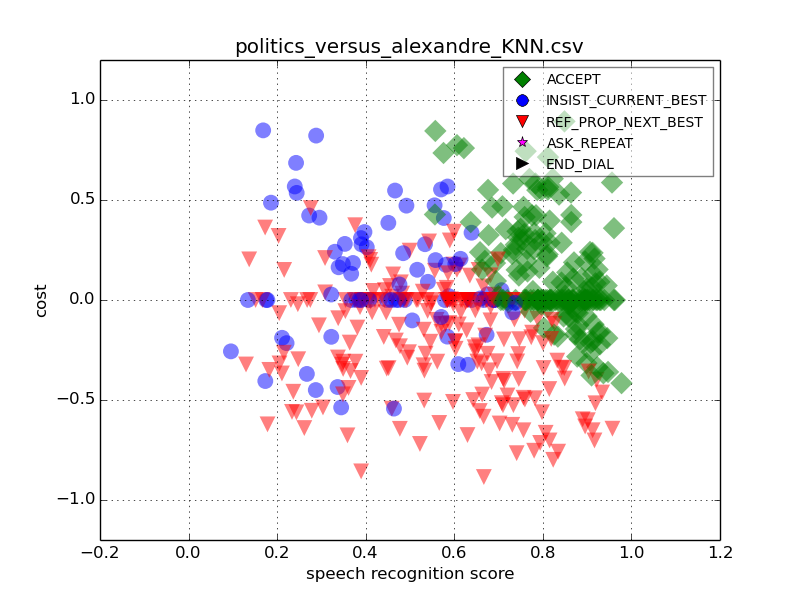
\includegraphics[width=0.5\textwidth]{sources/contribution/sigdial/vsAlex.png}
    \label{fig:policies1}
    }
    \subfloat[\textit{vsWill policy's 2D projection.}]{
    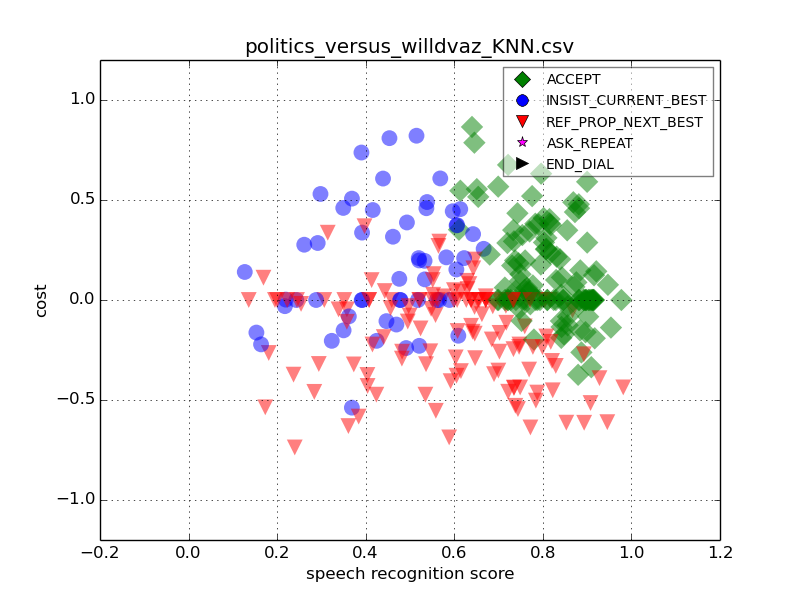
\includegraphics[width=0.5\textwidth]{sources/contribution/sigdial/vsWill.png}
    \label{fig:policies2}
    }\\
    \subfloat[\textit{vsNico policy's 2D projection.}]{
    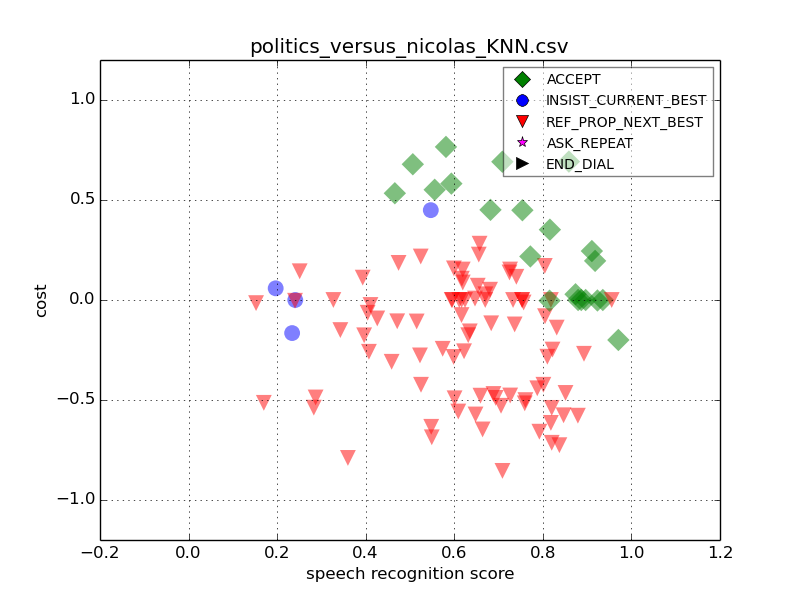
\includegraphics[width=0.5\textwidth]{sources/contribution/sigdial/vsNico.png}
    \label{fig:policies3}
    }
    \caption{Some projections of policies optimised versus human-model users}
    \label{fig:projection}


\end{figure}
\begin{figure*}
    \begin{center}
        \subfloat[\textit{Overall returns (handcrafted)}]{
        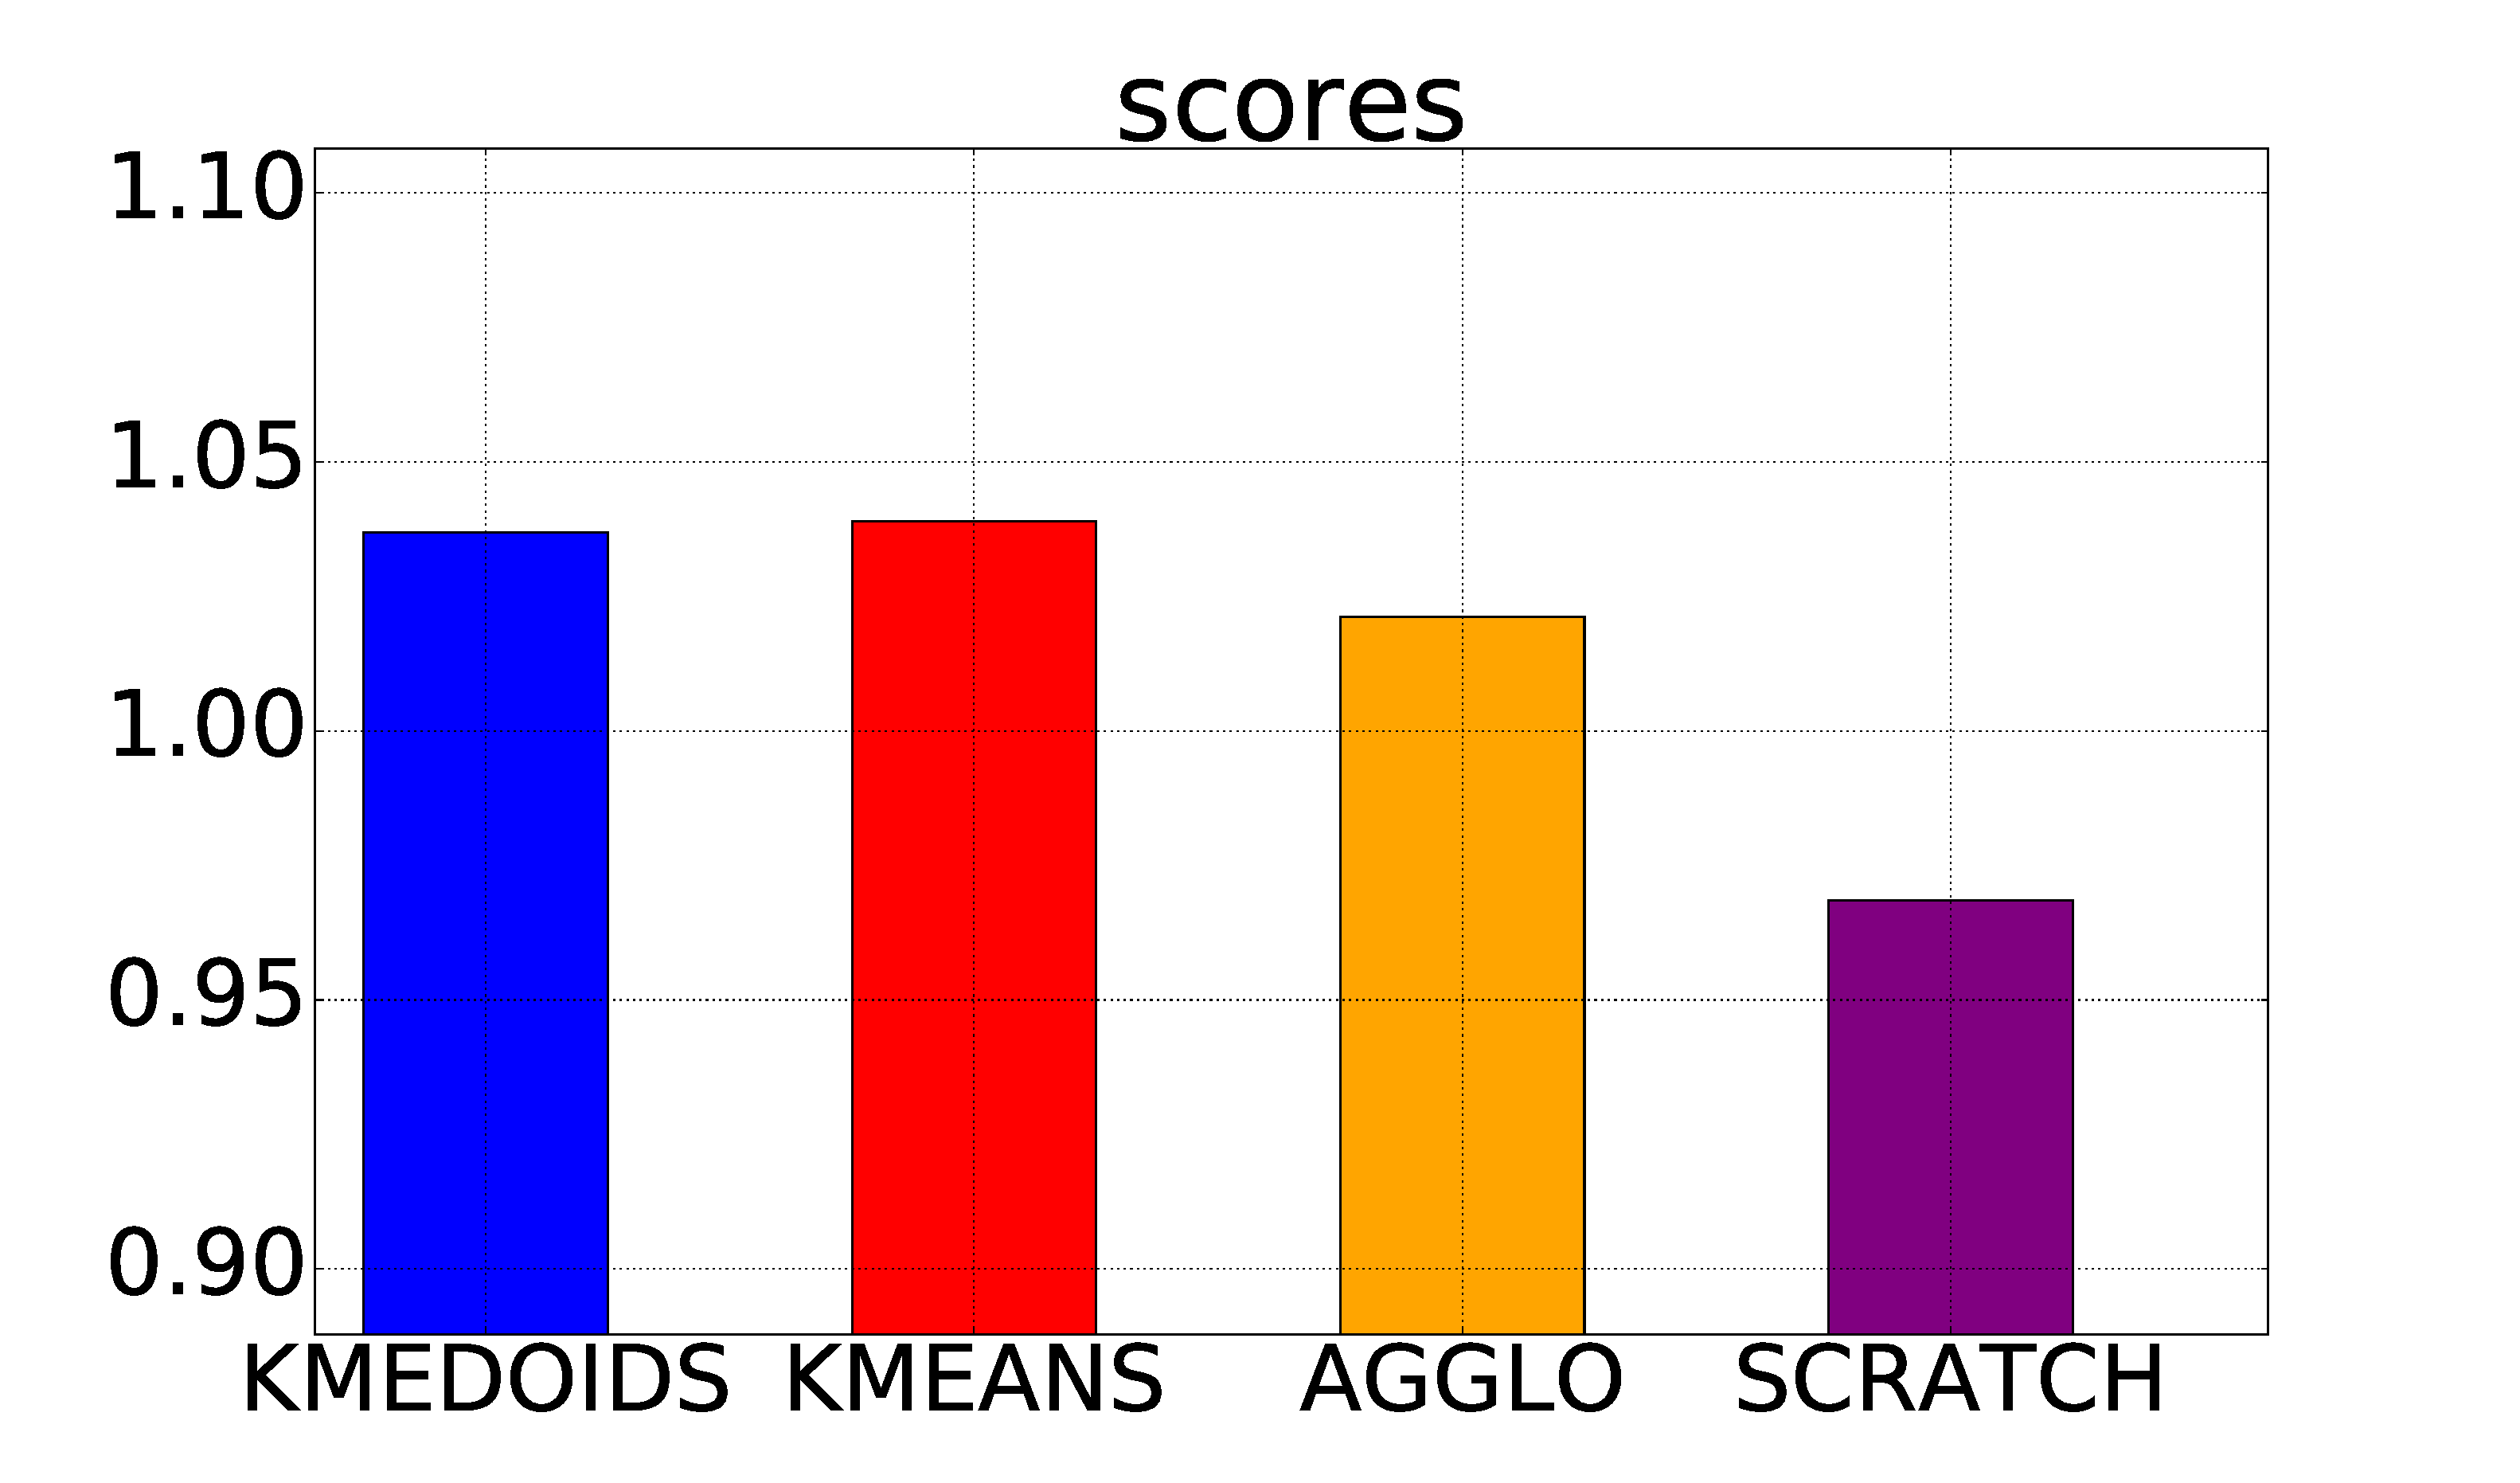
\includegraphics[width=0.33\textwidth]{sources/contribution/sigdial/handcraftedScores.pdf}
        \label{sub:handcraftedScores}
        }
        \subfloat[\textit{Dialogues lenghts (handcrafted)}]{
        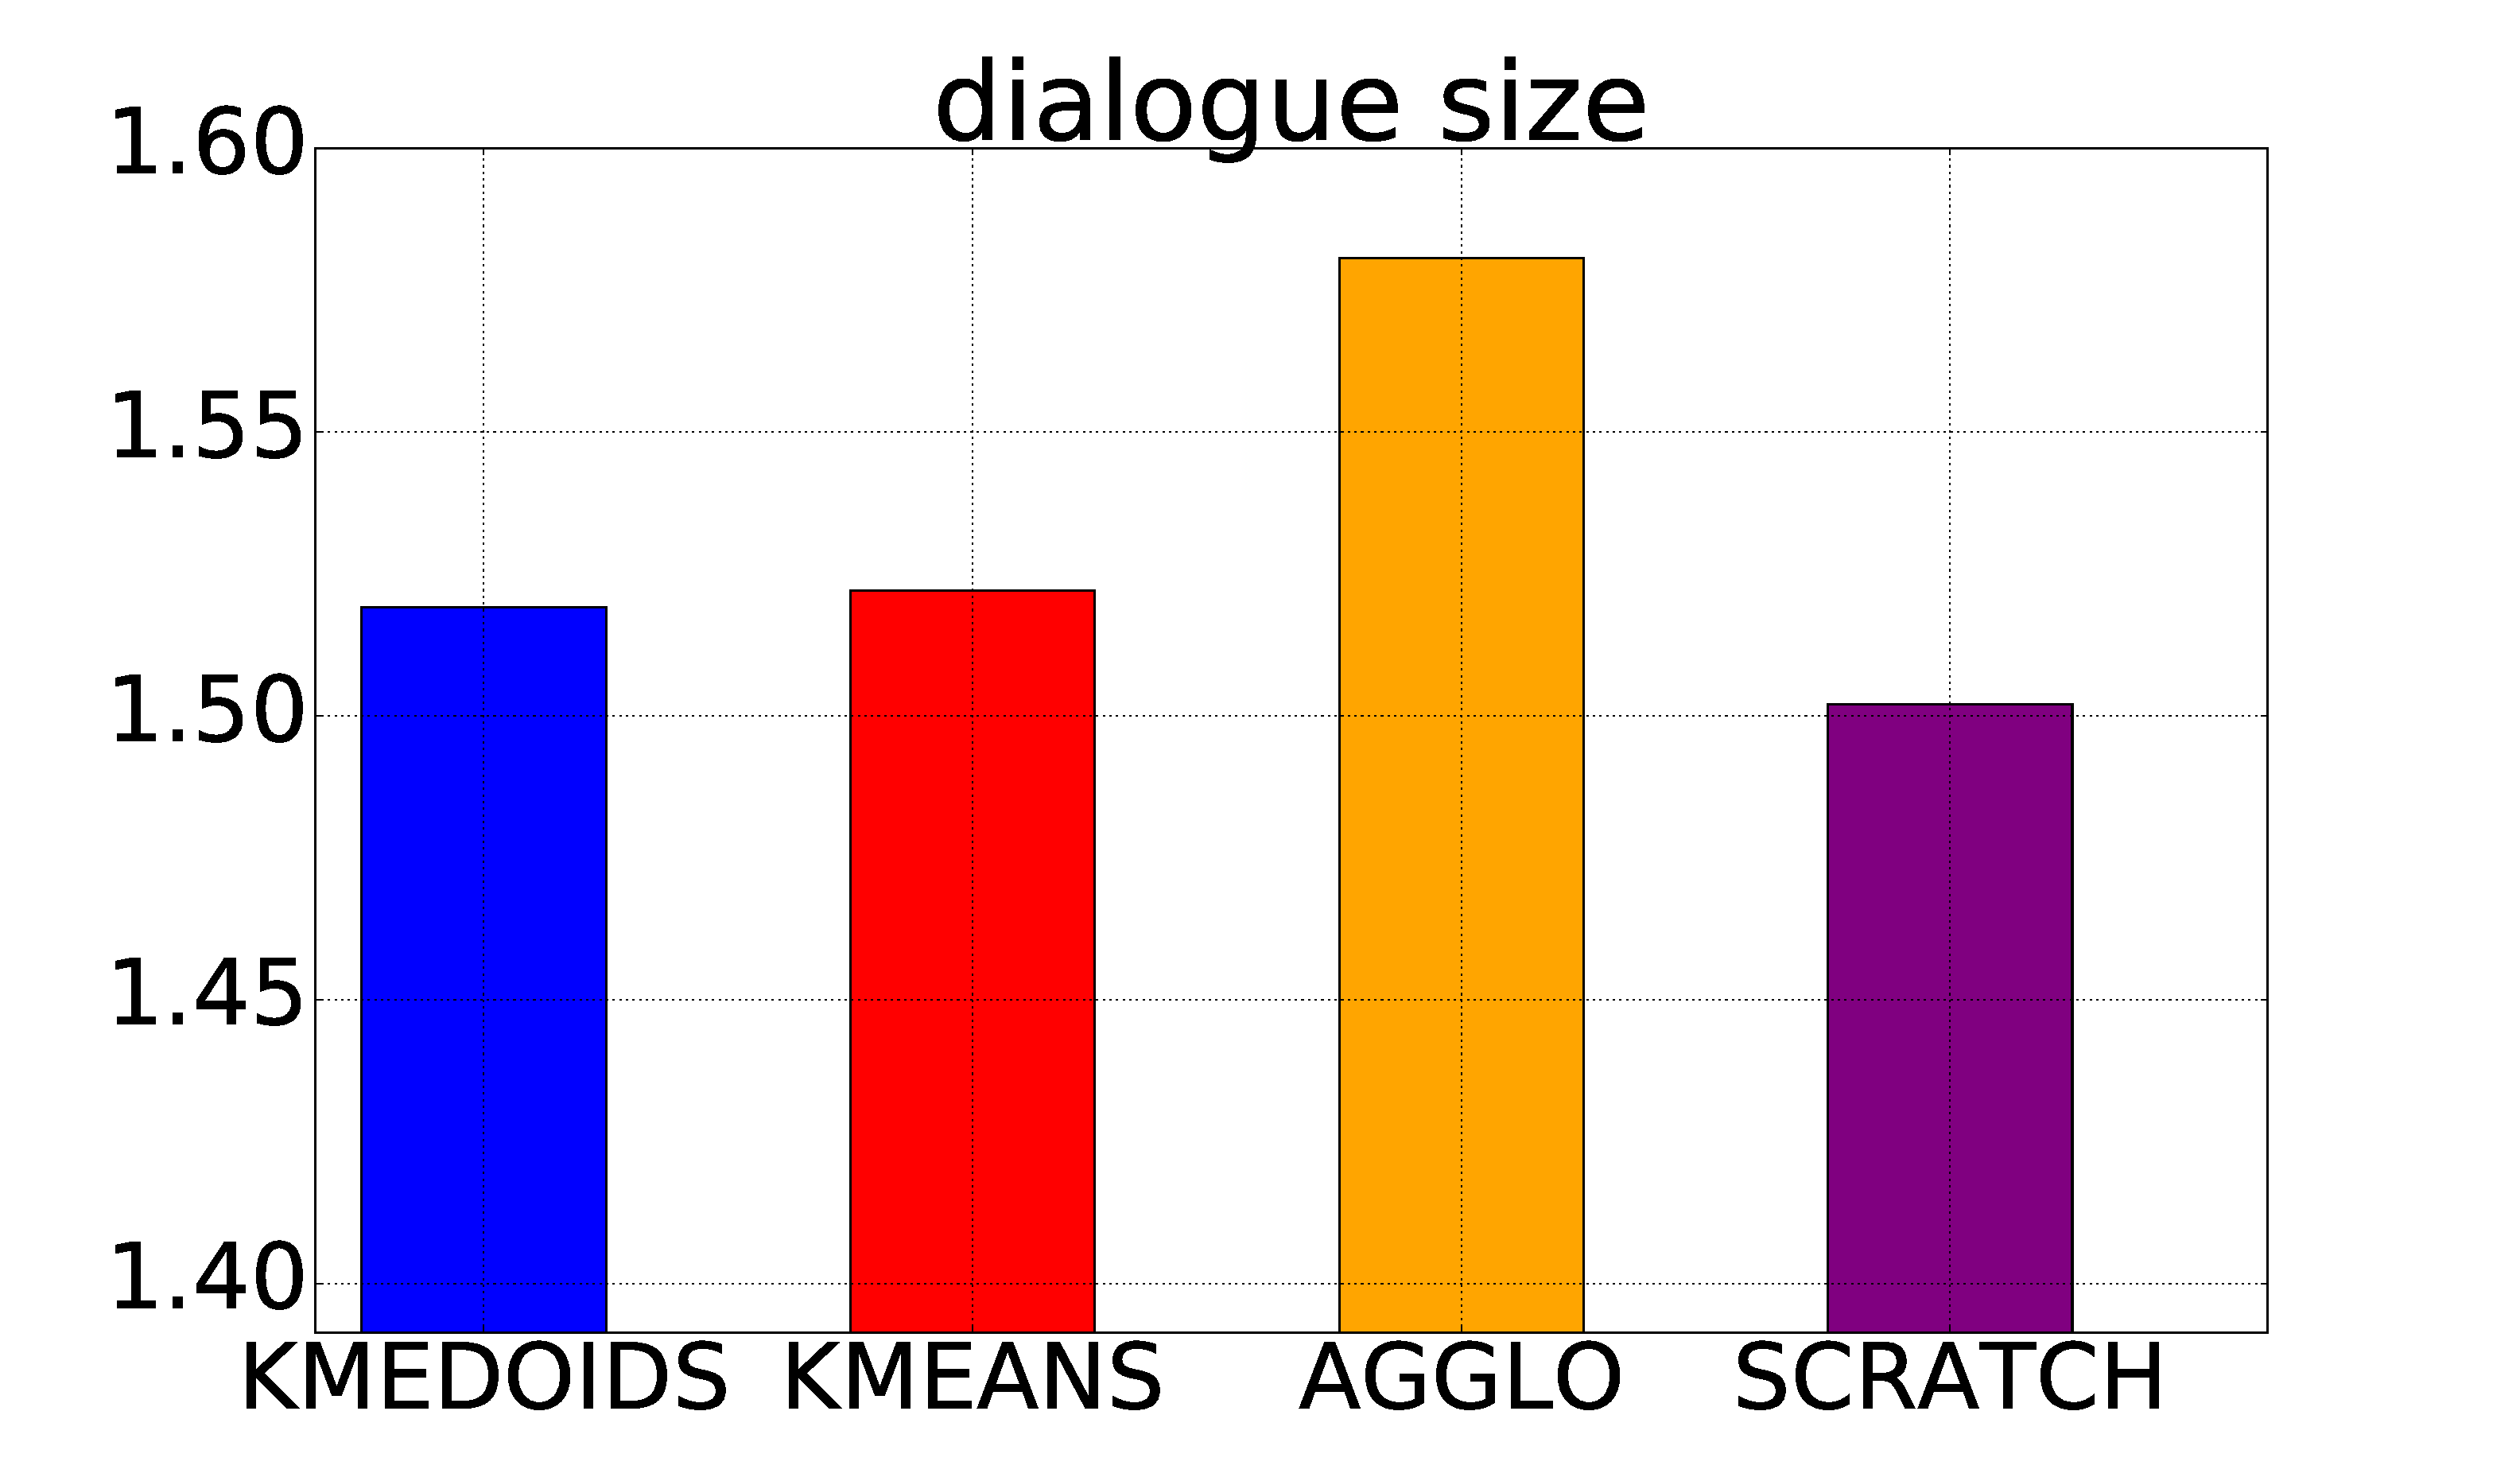
\includegraphics[width=0.33\textwidth]{sources/contribution/sigdial/handcraftedDialoguesize.pdf}
        \label{sub:handcraftedDialoguesize}
        }
        \subfloat[\textit{Task completion in \%  (handcrafted)}]{
        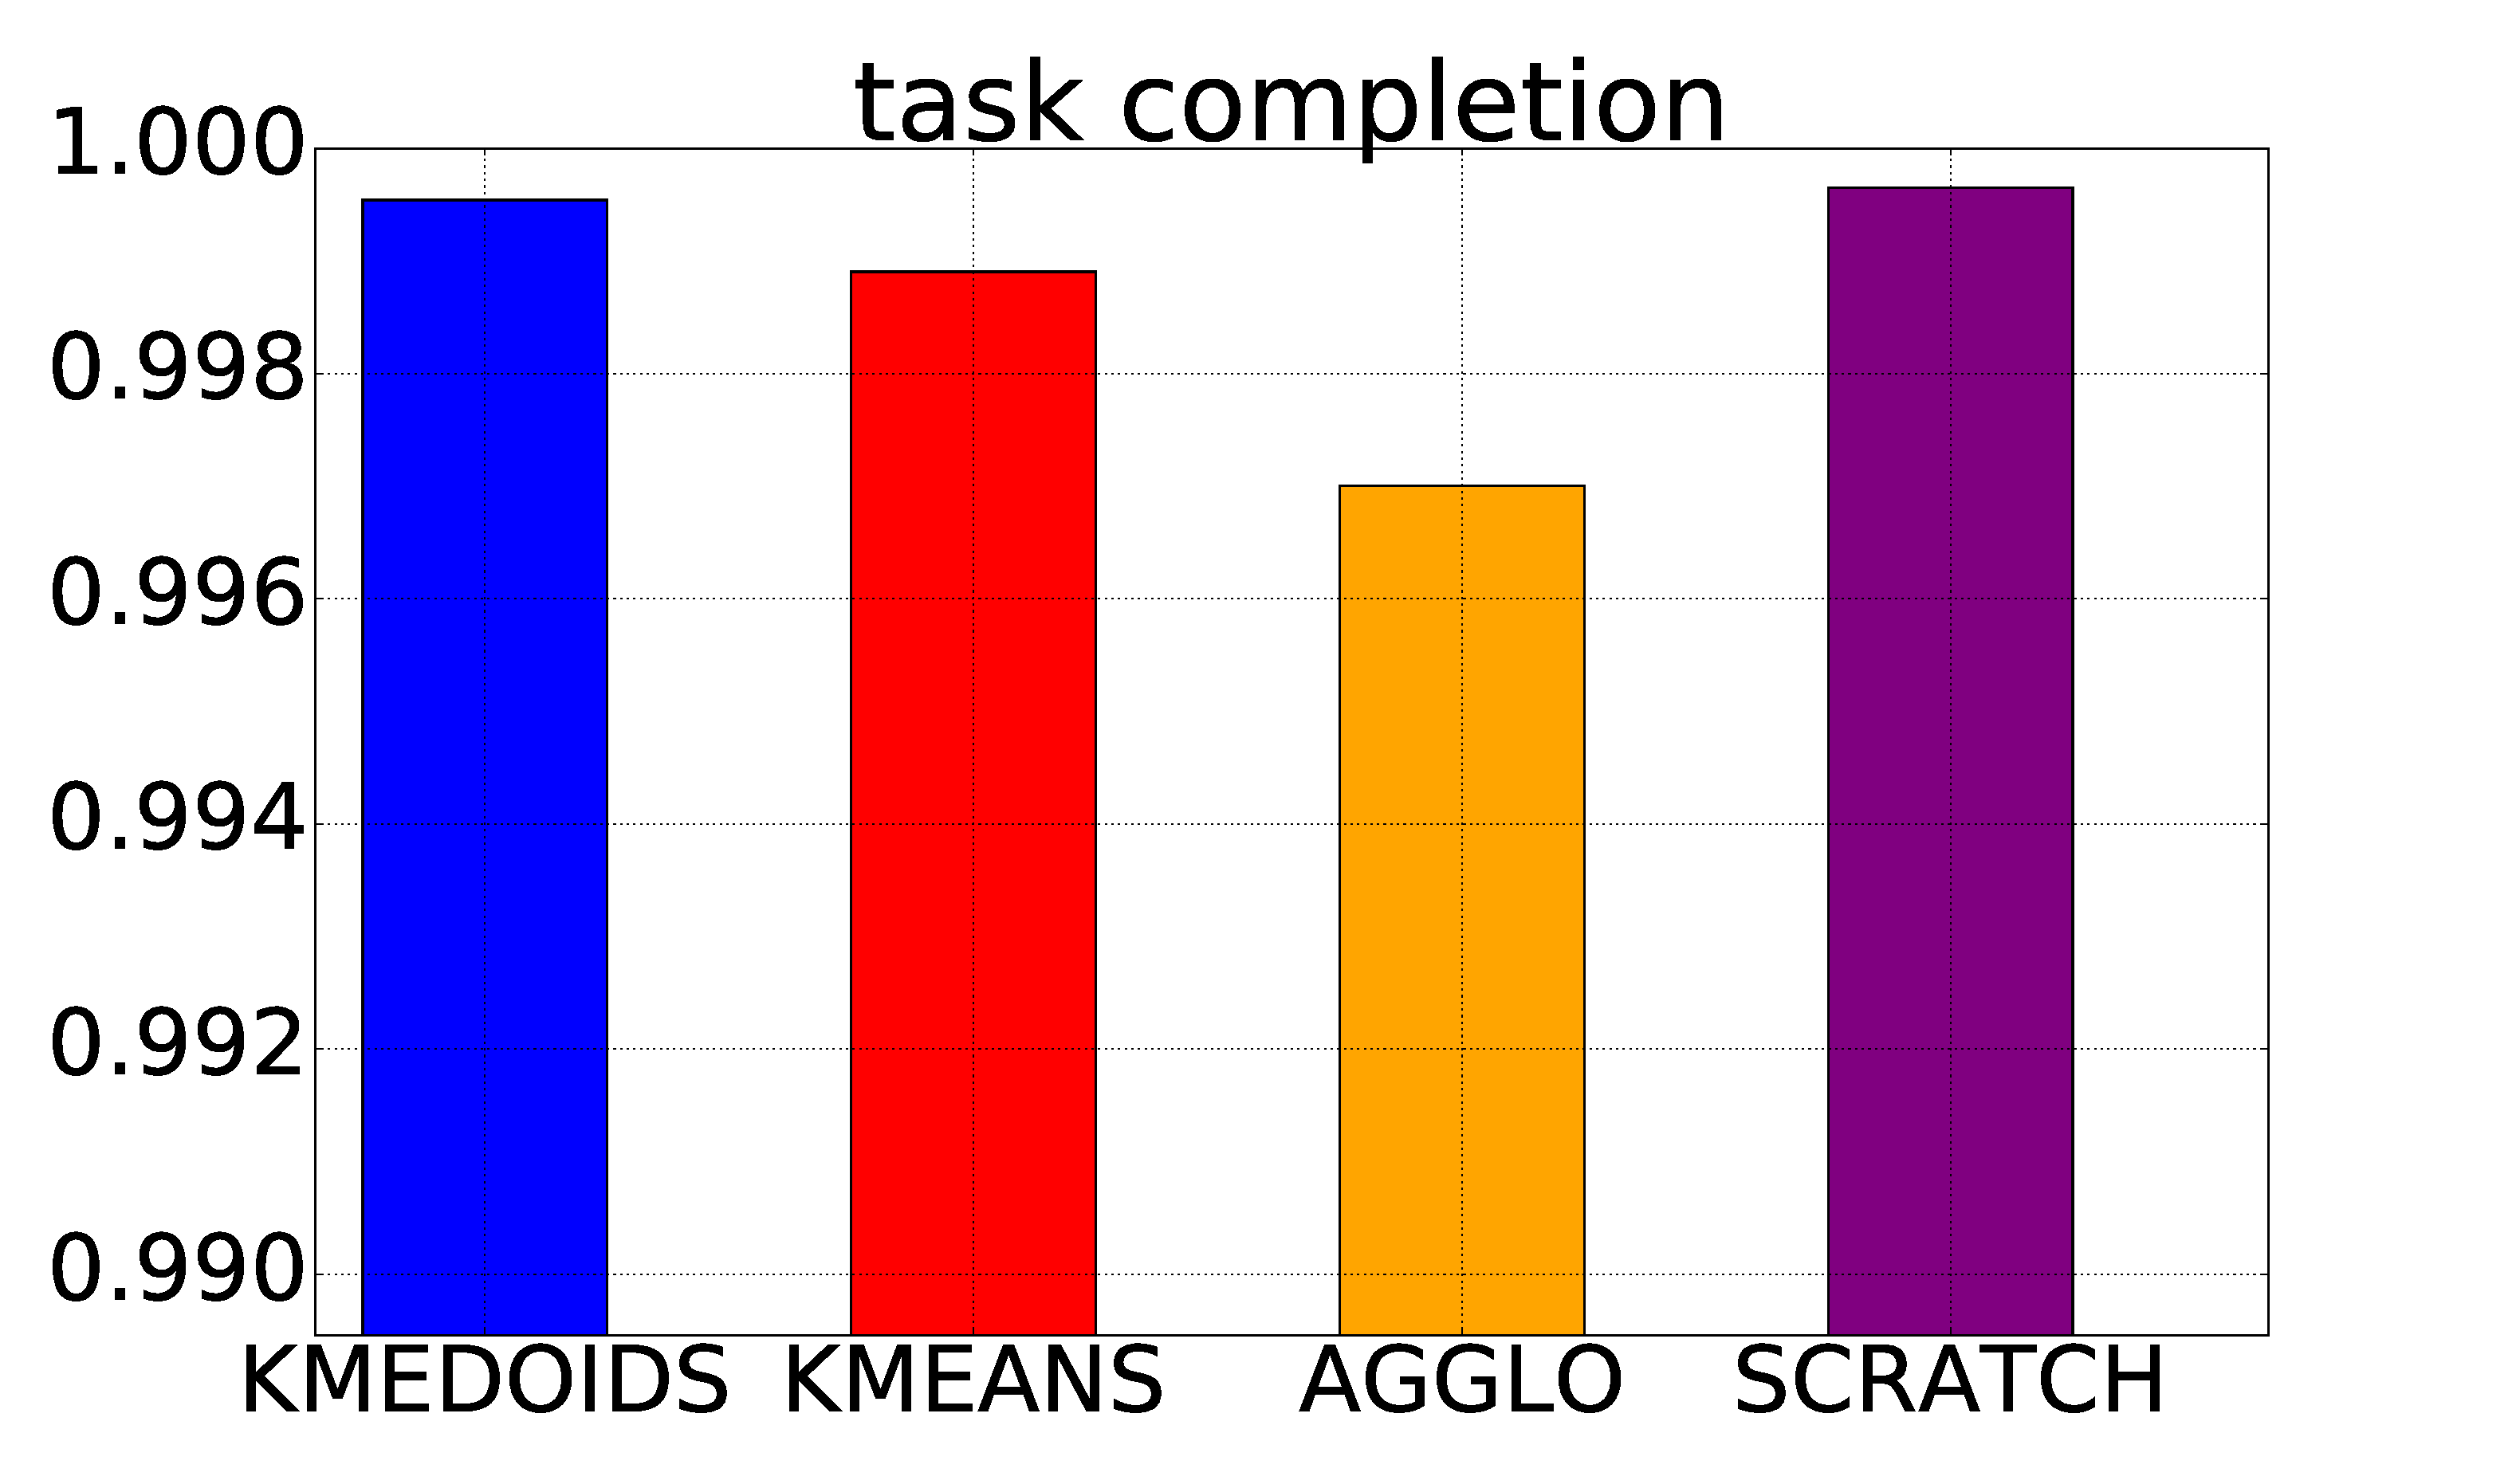
\includegraphics[width=0.33\textwidth]{sources/contribution/sigdial/handcraftedTC.pdf}
        \label{sub:handcraftedTC}
        }    \\
        \subfloat[\textit{Overall returns (human)}]{
        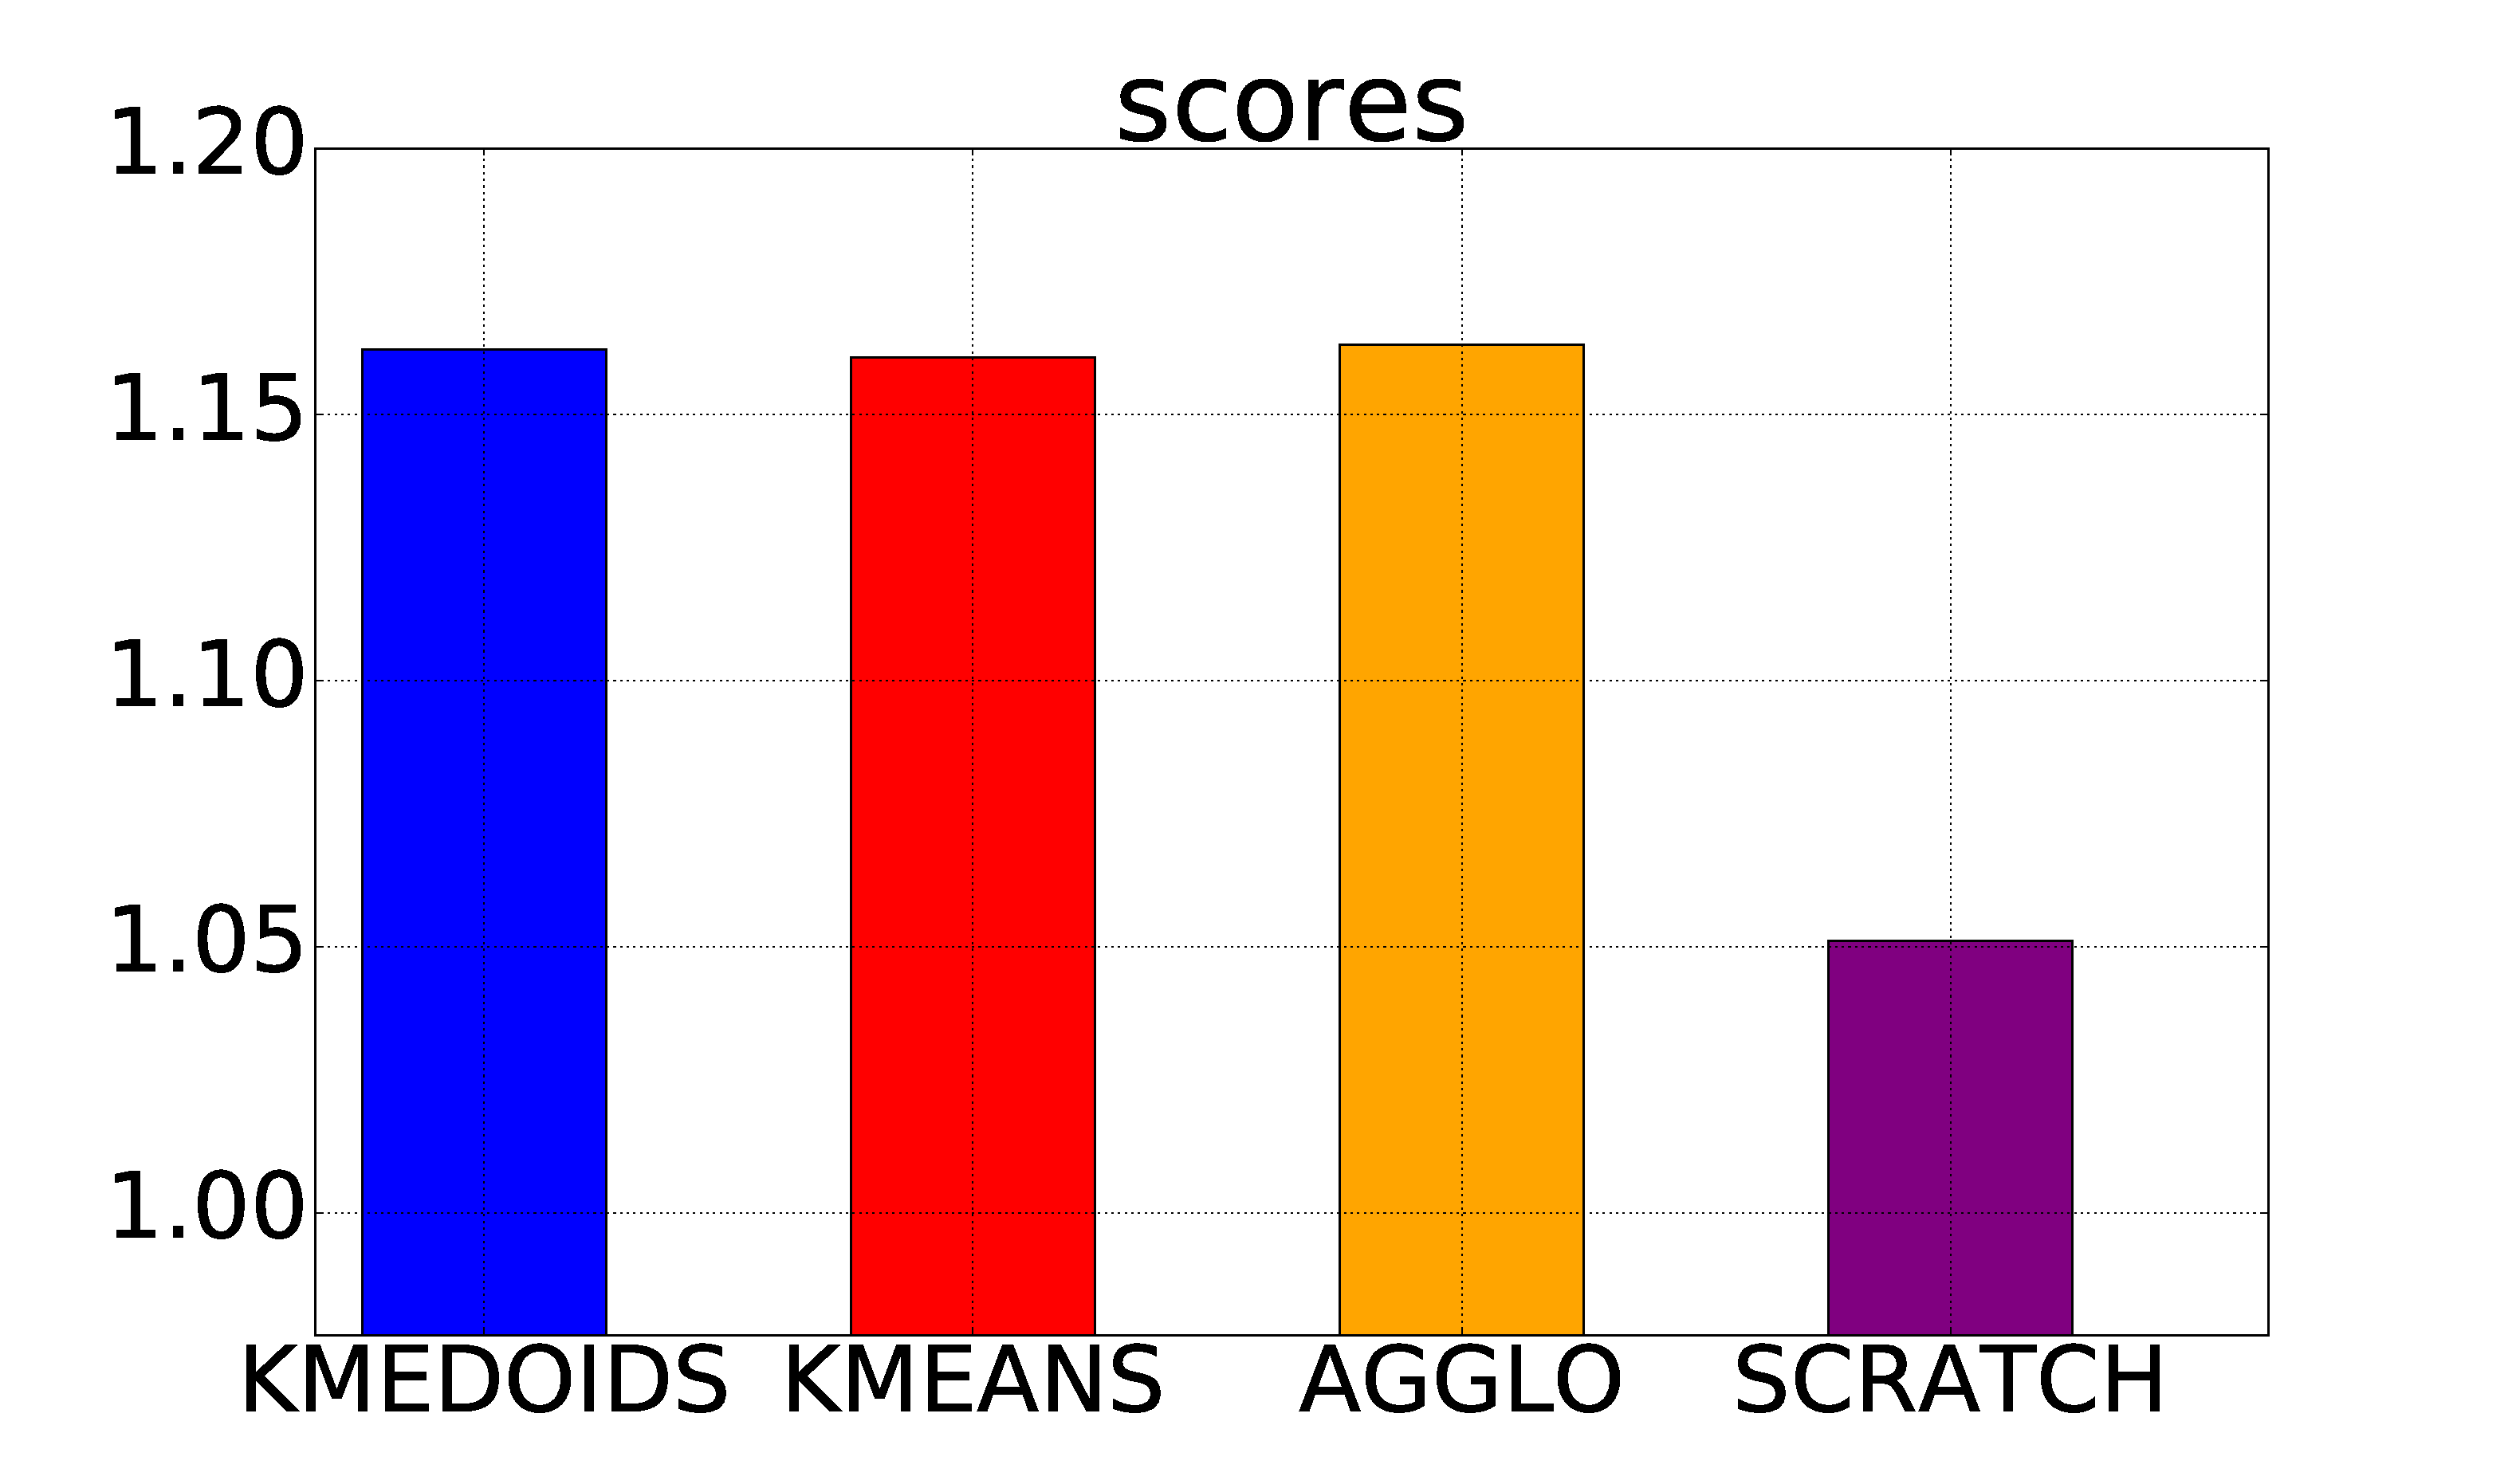
\includegraphics[width=0.33\textwidth]{sources/contribution/sigdial/humanScores.pdf}
        \label{sub:humanScores}
        }
        \subfloat[\textit{Dialogues lenghts (human)}]{
        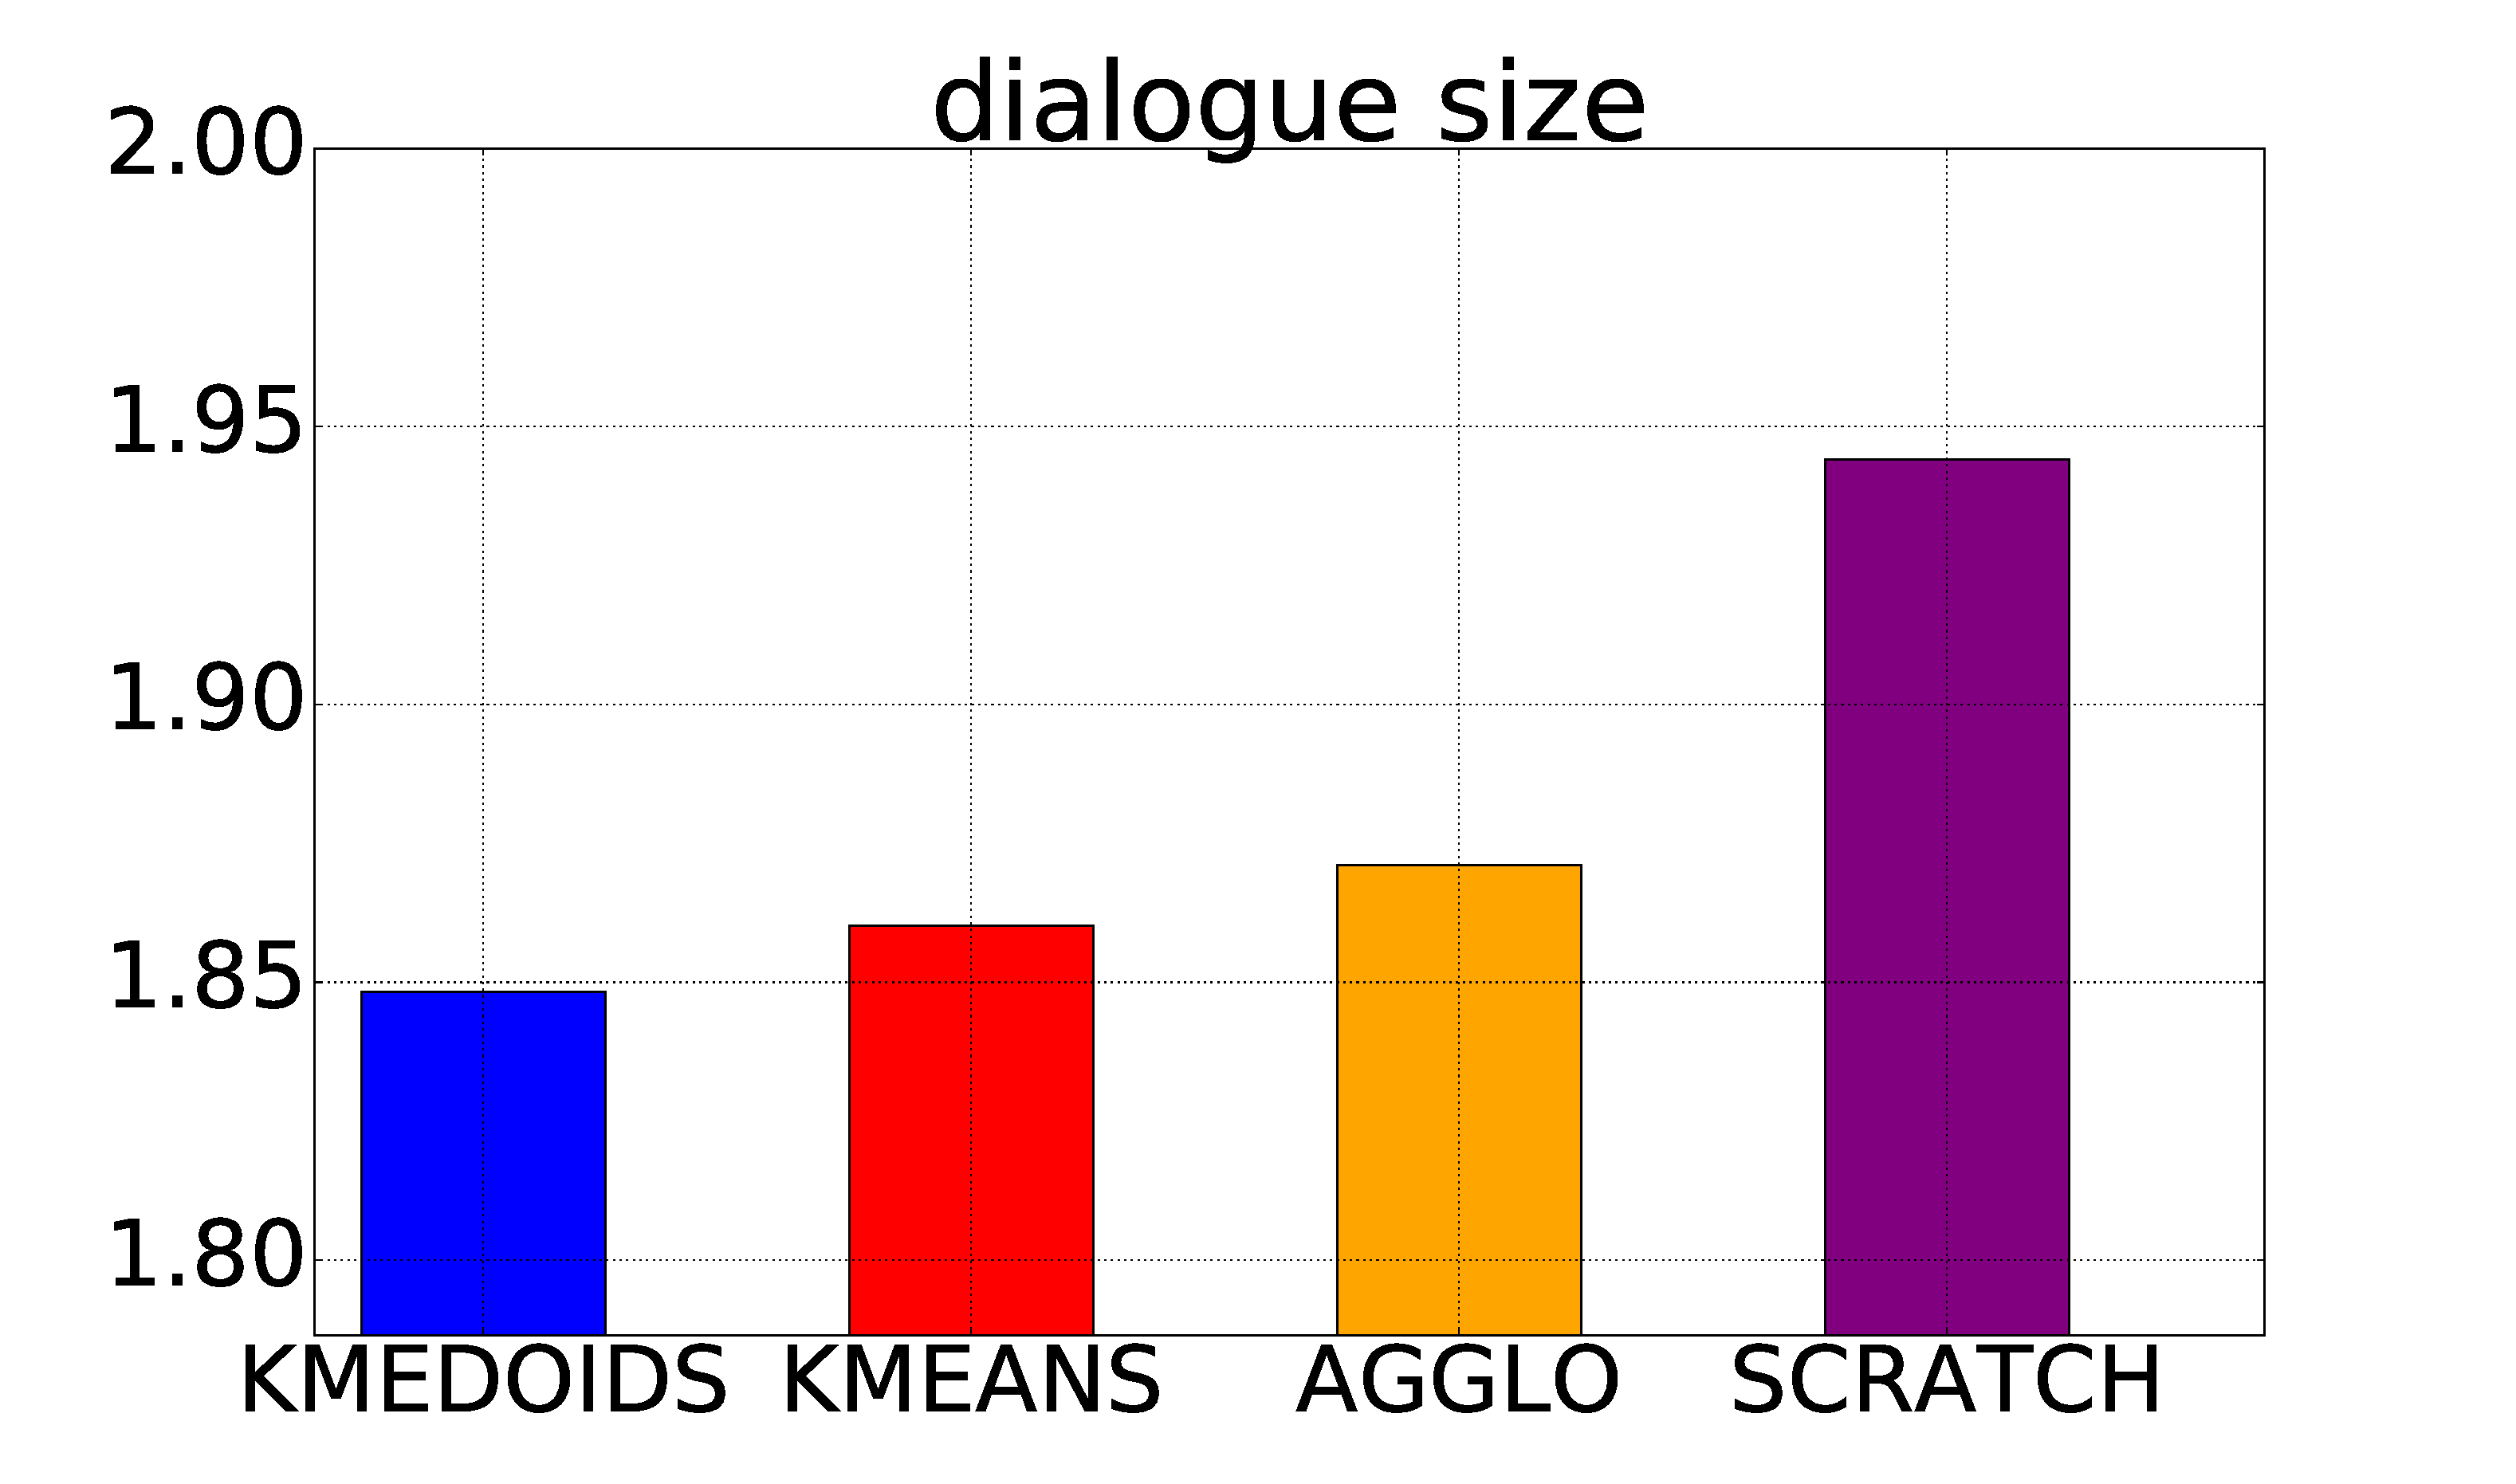
\includegraphics[width=0.33\textwidth]{sources/contribution/sigdial/humanDialoguesize.pdf}
        \label{sub:humanDialoguesize}
        }
        \subfloat[\textit{Task completion in \% (human)}]{
        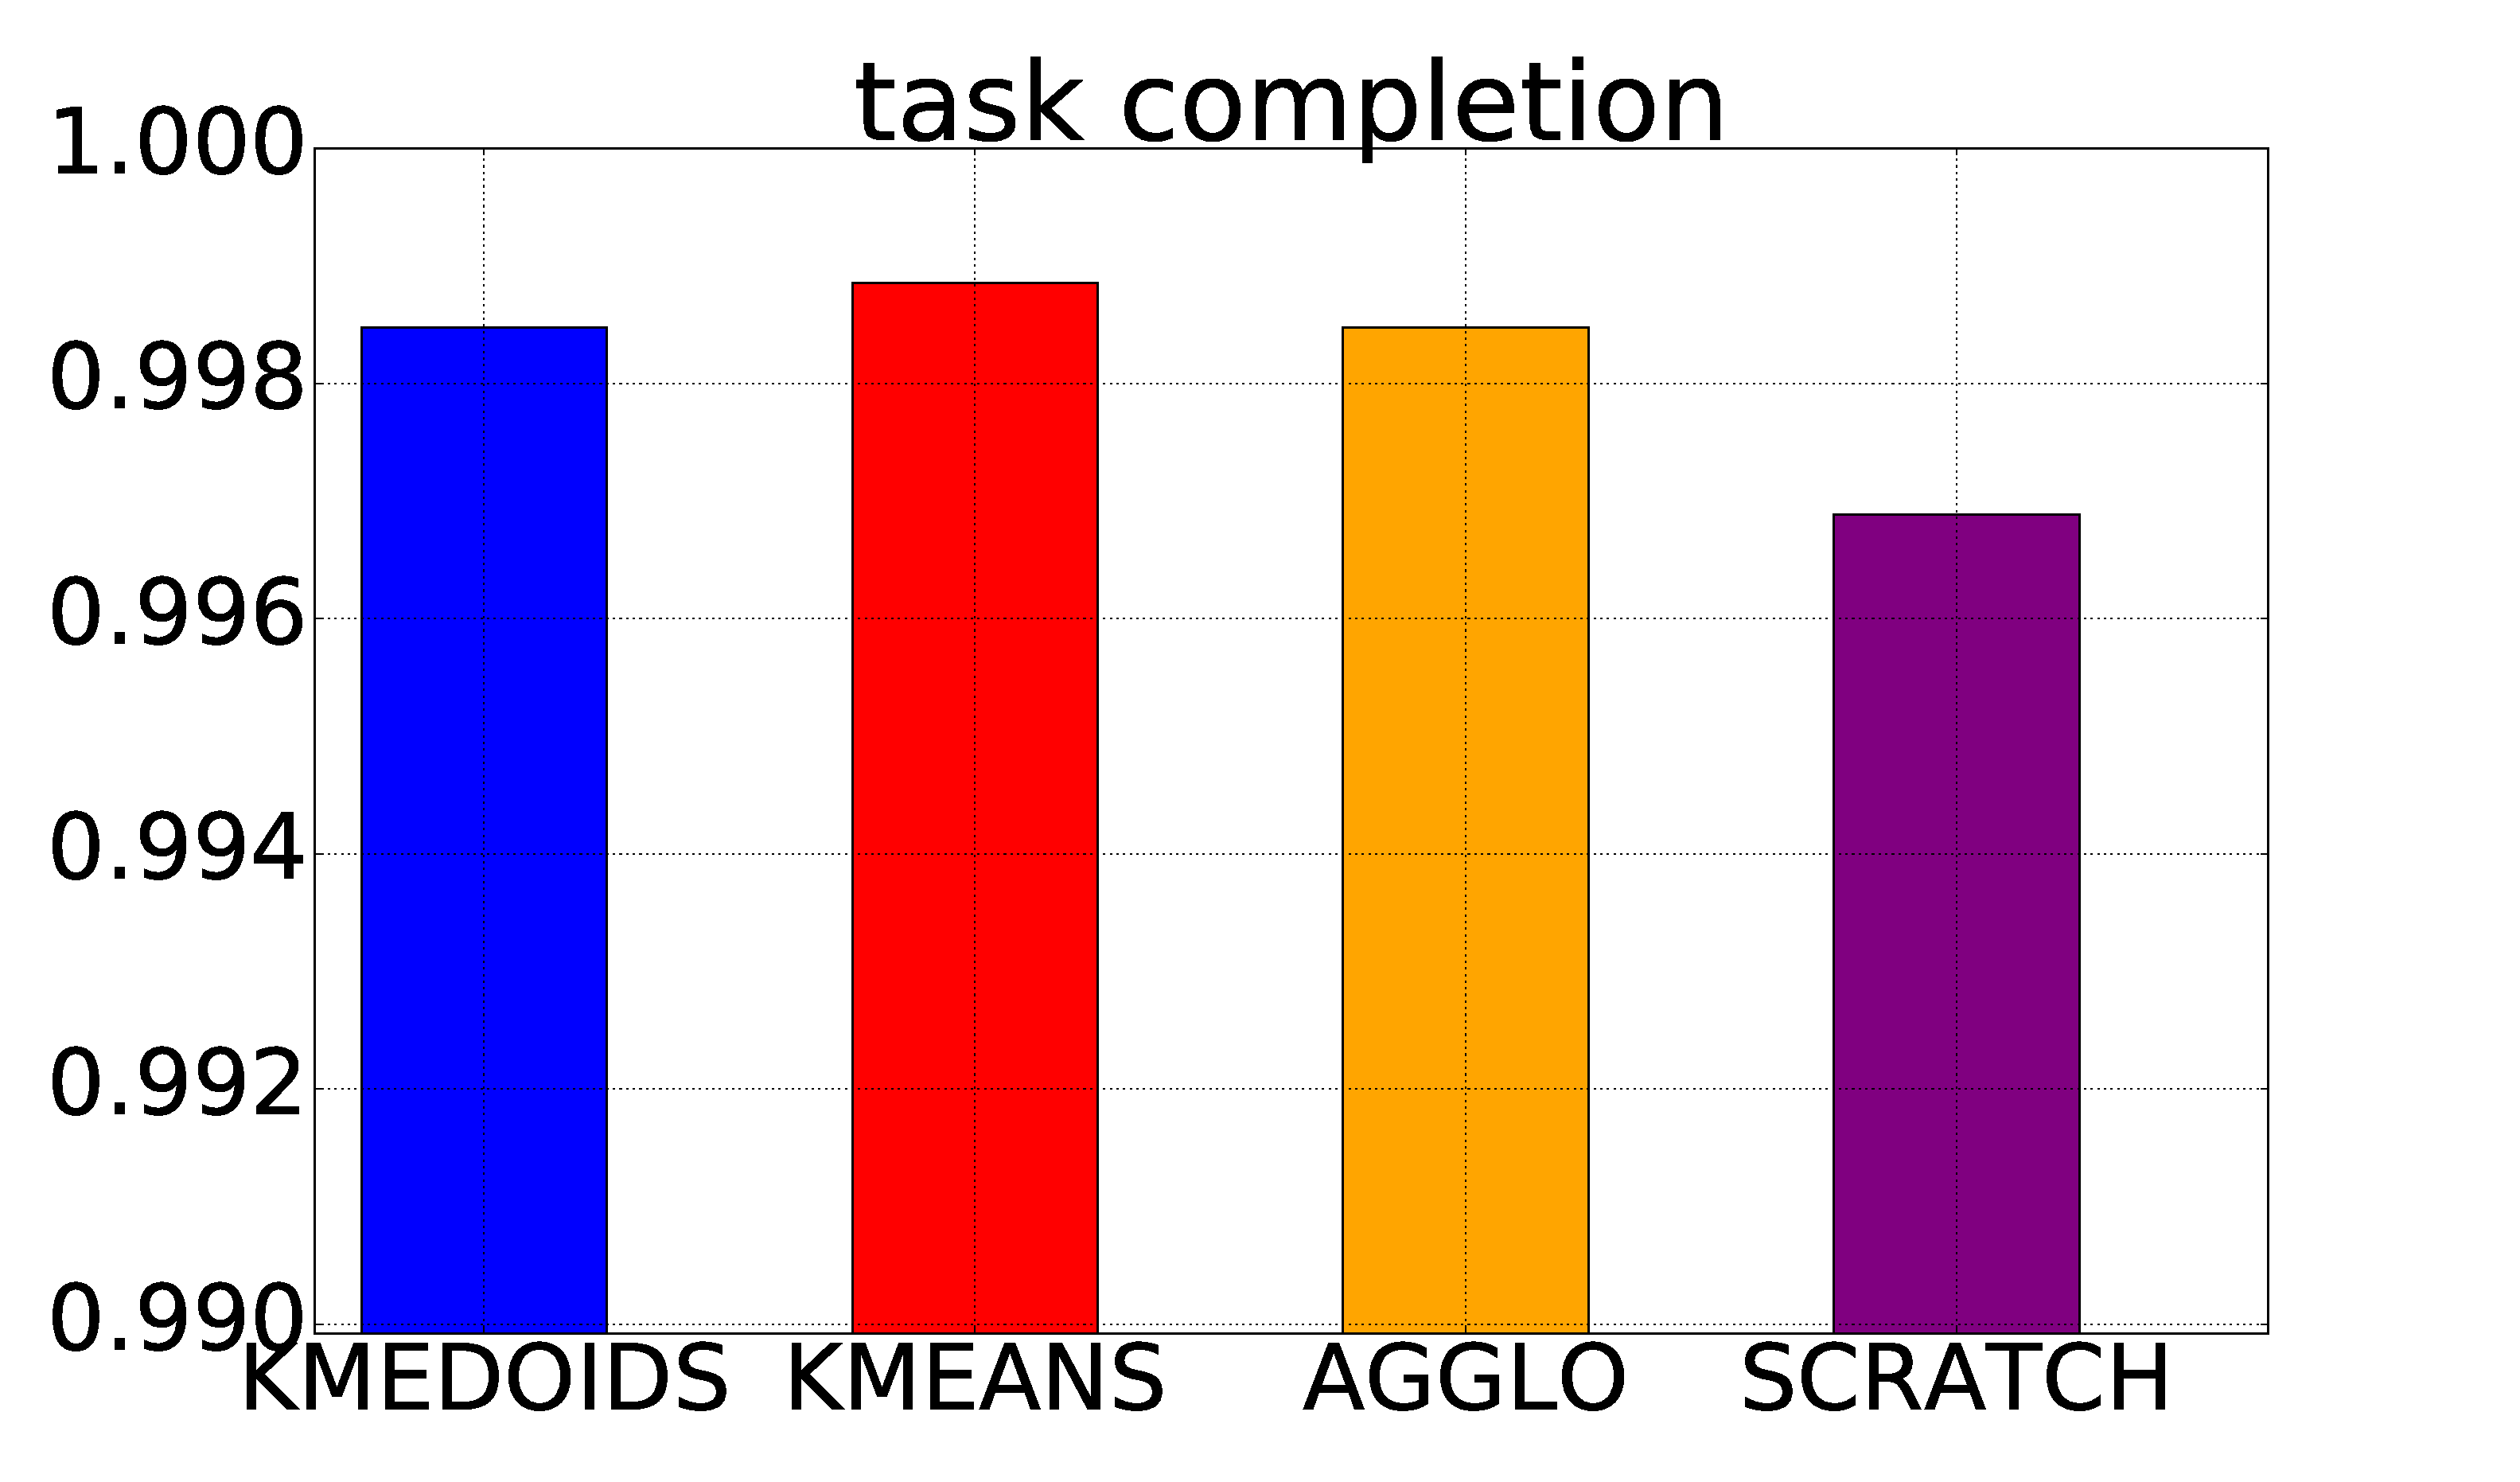
\includegraphics[width=0.33\textwidth]{sources/contribution/sigdial/humanTC.pdf}
        \label{sub:humanTC}
        }
        \label{fig:human}

        \caption{Dialogue quality in the handcrafted and human setup}
        \label{fig:handcrafted}
    \end{center}
\end{figure*}
To show the importance of \idx{user adaptation}, source systems are respectively trained versus \idx{user}s. Then, each system interacts with all the \idx{user}s and we compare the results. The experiences are repeated for 10 runs. Dialogue\index{dialogue} testing size is set to $10^3$ for each run. In the \textbf{\idx{handcrafted} setup}, as in \textcite{Genevay2016}, \idx{handcrafted user}s are created. Parameters of these \idx{user}s are listed in \Cref{fig:cchandcrafted}. Also, cross comparisons between source \idx{user}s and systems are displayed. Results in bold show that each system trained versus a specific \idx{user} is the best fit to \idx{dialogue} with this \idx{user}. One can see clear similarities between some of the results. This is where the representatives design method will operate by grouping all these similar policies.

In the \textbf{human setup}, test systems are trained against the \idx{human-model user}. Results are shown in \Cref{fig:cchumanmodels}. Note that label \textit{Will} means \idx{model} of \textit{Will} and not \textit{Will} himself as well as \textit{vsWill} means the system trained against \textit{Will}'s \idx{model}. Again, trained systems perform better than others against the \idx{user} they learnt on. However, differences are not as clear as in the \idx{handcrafted} setup. The reason is shown in \Cref{fig:policies1}, ~\ref{fig:policies2} and ~\ref{fig:policies3} where learnt policies are quite similar. Computed policies are tested on the states $s_{\indextransition}$  from the set of $(s_{\indextransition},a_{\indextransition},r'_{\indextransition},s'_{\indextransition})_{\indextransition \in \T}$ they learnt from. The $(\srs,c)$ projection explains better \idx{policy} differences. One can see that \textit{vsAlex} and \textit{vsWill} are pretty similar as they insist often when the cost is negative, in contrary of other policies. On the other hand, \textit{vsNico} tends to \texttt{RefProp} instead of \texttt{Accept} when the \gls{SRS} is high. It is straightforward to remark that this is because \textit{Nico} has tendencies to \texttt{Accept} more than others as we saw in \Cref{actionsdistrib}.
One can notice that even if statistics gathered from human actions distribution shows significant differences (in \Cref{actionsdistrib}), computed policies are not necessarily different (like \textit{vsAlex} and \textit{vsWill}).

\subsection{Adaptation results}
\label{subsection:adaptationprocess}

Now that specialised systems have been shown to lead to better results, we test the full adaptation process with \textsc{Kmedoids} and \textsc{Kmeans} methods.
%!TU: remarque habituelle sur le style direct(we)/indirect: choisi ton camp !!
As previously, we performed tests on both \idx{handcrafted} and human-model users\index{human-model user}. But first, the database of source systems is constructed. We created 100 source handcrafted users\index{handcrafted user} and 100 source human-model users\index{human-model user}. Those are designed by changing some parameters of the vanilla \idx{user}s. For example, a \idx{model} from Alex is changed switching its \gls{SER} ($\ser$) from 0.3 to 0.5. Parameters take random value between the following intervals: $\mutop\in[0,5]$ with $\mubot=-\mutop$, $\ser\in[0,0.5]$, $\cooperationrate \in[0,1]$, and $x\in [0.1,0.9]$. It is useful for human setup because we do not have enough \idx{dialogue corpora} to design 100 systems specialized versus 100 unique \idx{human-model user}s. The same method is applied to generate a large number of \idx{handcrafted user}s as well. For each \idx{user}, a source \idx{policy} is trained after 6 batches\index{batch} of 200 \idx{dialogue}s\index{dialogue} (for a total of 1200 \idx{dialogue}s\index{dialogue}). Each system is added to its respective database (human-model\index{human-model user} or handcrafted\index{handcrafted user}). We end up with 100 source trained policies\index{policy} with 100 source \idx{handcrafted user}s  and 100 source trained policies\index{policy} with 100 \idx{human-model} source \idx{user}s.

\textsc{Kmeans} and \textsc{Kmedoids} are tested for the complete adaptation process versus a base of 500 target \idx{user}s generated randomly (in the same way as \idx{user}s have been generated to create source systems). As discussed in \Cref{sec:adapatationframework}, the adaptation process implies a bandit phase: 25 \idx{dialogue}s are done versus the target \idx{user} then the mean return is saved to be plotted. Then all the \idx{transition}s $(s, a, r', s')$ are retrieved from the source system winner of the bandit. The process actually \idx{transfer}s a maximum of 1200 \idx{dialogue}s. Transfer \idx{transition}s are submitted to a filtering using Density-Based selection with $\eta$ parameter picked in the set $\{0.1,0.3,0.5,0.7,0.9\}$ \footnote{We kept only $\eta=0.3$ as results are pretty similar with any $\eta$}. Then, a new \idx{policy} is learnt with \gls{FTQ} fed with \idx{transition}s from the source system and \idx{transition}s from the bandit \idx{dialogue}s. To avoid divergence, a $\lambda$-regularisation~\parencite{Tikhonov1963,Massoud2009} is applied to \gls{FTQ} with $\lambda=1$. Once the \idx{policy} learnt, 25 additional \idx{dialogue}s are sampled versus the target \idx{user}. After this sampling, the mean return is saved to be plotted later. The process is repeated 6 times for a total of $25+6\cdot 25+1200$ \idx{dialogue}s maximum for the learning and $25+6\cdot 25+25$ \idx{dialogue}s for the evaluation. All systems, sources and targets, share the following parameters; $\omega=1$, $\discountfactor_u=0.9$, $\ser=0.0$, $\mutop=5$, $\mubot=-5$, $\cooperationrate=1$  but differ in their \idx{policy}. All systems are learnt with \gls{FTQ} using the following parameters: $\deltastoppingcriterion=0.001$, $\maxiteration=200$ and $\discountfactor=0.9$. They all follow an \idx{$\egreedy$-greedy} \idx{policy} with $\egreedy$ defined as in \Cref{subsection:systemdesign}.

In order to compare the previous methods, we introduce two naive ways for \idx{user adaptation}, \textsc{Agglo} and  \textsc{Scratch}. The first one learns a unique system to represent the whole systems database and the second one adopts a random \idx{policy} during the bandit phase then follows an \idx{$\egreedy$-greedy} \idx{policy} like other methods but without any \idx{transfer}.
%!TU:
%
Before running experiment, pre-processing is done for some the methods: for \textsc{Agglo}, 1200 \idx{dialogue}s are gathered among all source systems in the database. That means 12 \idx{dialogue}s are collected randomly from the \idx{dialogue} set of each of the 100 source systems. A \idx{policy} is learnt with one \idx{batch} of \gls{FTQ} with $\deltastoppingcriterion=10^{-6}$, $\discountfactor$=0.9 and $\maxiteration$=200. This \idx{policy} is used to create one unique system representative for all the database. For \textsc{Kmeans}, \textsc{PD-Distance} vector representations of each system in the database are created by sampling over 20000 states (picked from source systems). Then these systems are clustered with $k$=5 using $k$-means with euclidean distance. For each cluster the previous \textsc{Agglo} method is applied in order to create a cluster representative. Finally, for \textsc{Kmedoids}, a random sampling of five-element sets is ran. The $J$ value of each set is computed and the one who minimizes this value is kept. Finally, 10 different sets of \textsc{Agglo}, \textsc{Kmeans} and \textsc{Kmedoids} are created and tested. Results are shown in \Cref{fig:handcrafted}. In the \idx{handcrafted} setup, the overall \idx{dialogue} quality of the proposed methods is significantly better than \textsc{Agglo} and \textsc{Scratch} baselines. Indeed, \idx{dialogue}s are shorter \footnote{\textsc{Scratch}'s \idx{dialogue} size can be shorter because it use random \idx{policy} on \idx{jumpstart} and then ends the \idx{dialogue} more often.}, final return is higher and the task is more often completed. On the other side, returns and task completions are similar in the human setup. Still, the size of the \idx{dialogue}s is improved by \textsc{Kmeans} and \textsc{Kmedoids} offering a better \idx{dialogue} experience and thus \idx{user}s keep using the \gls{DS}.

\section{Related work}

To our knowledge, only one paper treats the subject of searching system representatives among a systems database:~\parencite{mahmud2013} has a similar adaptation process as the one presented in this chapter. It is not applied to \glspl{DS} specifically. In order to choose good representatives from the policies/MDP/systems database, \idx{clustering} is done using the following distance:
\begin{equation*}
    d_{\V(M_i,M_j)} = max\{\V_i^{\policy_i^*}-\V_i^{\policy_j^*},\V_j^{\policy_j^*}-\V_j^{\policy_i^*}\},
\end{equation*}
given two \glspl{MDP} $M_i$ and $M_j$, where $\V_k^{_{\policy}}$ is the return of the \idx{policy} $\policy$ when executed on \gls{MDP} $M_k$ and $\optimalpolicy_k$ refers to the optimal \idx{policy} for \gls{MDP} $M_k$. Thus, to compute all the systems distances two by two, one needs to sample \idx{dialogue}s between the source \idx{user}s and all the source systems of the database. In a real life \idx{dialogue} applications with humans, it is not possible to do such a thing unless one creates a \idx{model} of each source \idx{user}.

\section{Conclusion}
%
% TU: insiste un peu plus sur pouquoi le jeu de negotiation est pertinent pour la question de l'adaptation

In this chapter, \idx{user adaptation} has been proved to improve \glspl{DS} performances when \idx{user}s adopt different behaviours. The chapter shows that indeed, each human adopts a different way to play the \gls{NDG} although the shade is subtle. So, a system learnt versus a particular \idx{user} is more efficient than other systems for this \idx{user}, in the \idx{handcrafted user} setup as in the \idx{human-model user} setup.

User adaptation\index{user adaptation} requires selecting source systems to \idx{transfer} knowledge. This chapter proposed 2 methods: \textsc{Kmeans} and \textsc{Kmedoids} combined to a novel distance \textsc{PD-Distance} to select representative source systems, from a large database, which are used for \idx{transfer}ring \idx{dialogue} \idx{transition}s. These methods outperform generic policies in the \idx{handcrafted} setup and improve \idx{dialogue} quality when facing \idx{model}s learnt on human-human data.

In the next chapter, we will propose solutions to condense the whole pipeline into a single procedure, by extending the famous \gls{DQN} algorithm.
